\chapter{Level Statistics and Random Matrices}\label{ch:level-statistics}

\begin{chapterintro}
In the 1950s, nuclear physicists measuring how heavy nuclei absorb slow neutrons found long lists of sharp resonances. Each resonance is an energy level of a nucleus built from more than two hundred interacting protons and neutrons. Nobody could compute those levels one by one, and nobody can today. Eugene Wigner proposed a change of question. Instead of asking \emph{where} a particular level lies, ask \emph{how the levels are arranged}: how often two neighbors are unusually close together, how often they are unusually far apart. To answer that, he replaced the unknown Hamiltonian by a matrix with random entries and worked out the statistics of its eigenvalues. Those statistics matched experiment, and they turned out to depend on almost nothing except the symmetry of the problem \cite{mehta}.

About two decades later the same statistics appeared somewhere nobody expected. In 1972 the number theorist Hugh Montgomery had found a formula for how pairs of Riemann zeros are correlated, and Freeman Dyson recognized it as the formula for eigenvalues of random complex Hermitian matrices \cite{montgomery}. Andrew Odlyzko's computations then showed the agreement in great detail \cite{odlyzko87}. This is a large part of the reason physicists take the Hilbert--P\'olya idea (that the zeros might be the energy levels of some quantum system) seriously.

In this chapter you will learn how to measure the statistics of any spectrum: how to remove its changing density (unfolding), how to define the distribution of spacings between neighbors, and why uncorrelated levels give the law $e^{-s}$ while random matrices give laws that vanish at $s=0$ (level repulsion). You will derive the Wigner surmises completely, including the formula $\frac{32}{\pi^2}s^2e^{-4s^2/\pi}$ printed in the paper's Fig.~2, meet Montgomery's pair correlation, reproduce the paper's Fig.~2 with a few lines of Python, and finally see why consecutive fluctuations of the zeros are negatively correlated. \textbf{Where this shows up in the paper:} the evidence sentence of Sec.~I (Refs.~1--2 of the paper), the dataset check of Sec.~II A and Fig.~2, the unit of every rms in the paper, and the explanation in Sec.~III (paragraph ``Within-height splits'') of why smooth interpolation is anticorrelated with the truth.
\end{chapterintro}

\begin{prerequisites}
\item Chapter~\ref{ch:eigen}: eigenvalues of a $2\times2$ matrix from its characteristic polynomial; real symmetric and Hermitian matrices have real eigenvalues; the string (box) eigenvalues $(k\pi/2L)^2$.
\item Chapter~\ref{ch:counting-zeros}: the counting function $N(T)$, the smooth part $\Nsm(t)$ of paper Eq.~(1), the fluctuating part $S(t)$, smooth zeros $s_n$, the mean spacing $\gap_n$, fluctuations measured in mean spacings.
\item Chapter~\ref{ch:probability}: probability densities, mean, variance, standard deviation, rms, independence, the Gaussian and exponential distributions, histograms, Pearson correlation, autocorrelation of a sequence, random seeds.
\item Chapter~\ref{ch:series} (Taylor series of $\log(1-x)$, the geometric series) and Chapter~\ref{ch:complex} (modulus of a complex number).
\item First-year physics and calculus: integration by parts, substitution, the circumference $2\pi r$ of a circle and the surface area $4\pi r^2$ of a sphere.
\end{prerequisites}

%=====================================================================
\section{Spectra as patterns of points}\label{sec:level-statistics-patterns}

A spectrum is a list of numbers on a line: the energy levels $E_1<E_2<E_3<\cdots$ of a quantum system, or the heights $t_1<t_2<t_3<\cdots$ of the zeta zeros. You can ask two very different kinds of questions about such a list.

\textbf{Position questions} ask about individual members: where is level 500? Given levels 1--400, where are levels 401--500? This is the paper's central question. Its Fig.~1 is about positions.

\textbf{Statistical questions} ask about the pattern formed by many members, without caring which member is which: what fraction of neighboring pairs are closer than half the average distance? Is a large gap more likely to be followed by a small one? The paper's Fig.~2 is about statistics.

An analogy helps. Imagine three fields seen from above.
\begin{itemize}
\item In an orchard, trees stand in exact rows. Every gap between neighbors is the same. Physicists call such a spectrum a \textbf{picket fence}.
\item In a meadow, wildflower seeds have been scattered by the wind, each one landing independently of all the others. Some land almost on top of each other; some leave wide bare patches. This is a \textbf{Poisson} pattern (you met the Poisson process in Chapter~\ref{ch:probability}).
\item In a colony of nesting birds, each pair defends a little territory. Nests are never very close together, yet they do not form a perfect grid. This pattern shows \textbf{repulsion}.
\end{itemize}
Figure~\ref{fig:level-statistics-barcodes} shows three such patterns on a line. The middle one is a stretch of the Riemann zeros, after the rescaling (``unfolding'') that Sec.~\ref{sec:level-statistics-unfolding} explains. Even by eye you can see that the zeros behave like the birds: no pair is very close, and the gaps vary much less than in the Poisson row.

\begin{figure}[htbp]\centering
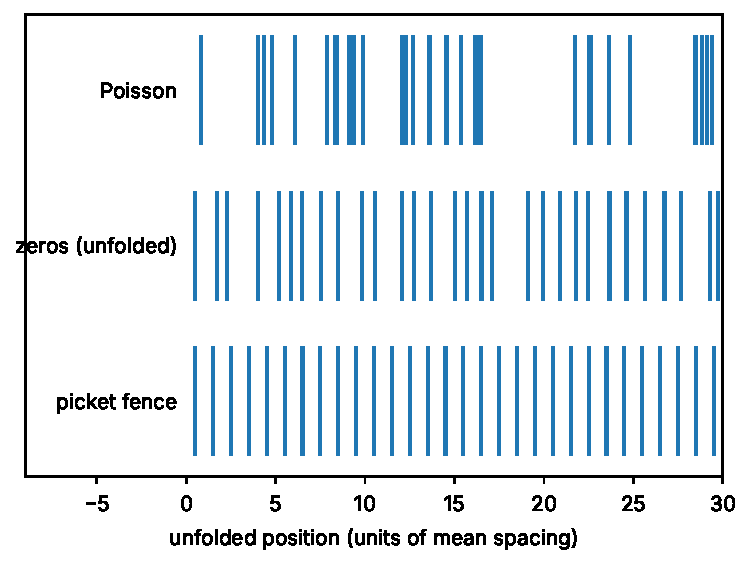
\includegraphics[width=0.85\linewidth]{figs/level-statistics_barcodes.pdf}
\caption{Three point patterns with the same average density (one point per unit length). Top: uniformly random independent points (Poisson); note the near-collisions and the wide empty stretches. Middle: the Riemann zeros starting at zero number 1001, unfolded so that their mean spacing is one. Bottom: a picket fence. The zeros avoid close pairs (level repulsion) without being regularly spaced.}
\label{fig:level-statistics-barcodes}
\end{figure}

Statistical questions have one great advantage: they can have universal answers. Two completely different systems can share the same statistics while having no individual level in common. That advantage is also a limitation, and it is central to the paper: matching the statistics of a spectrum says nothing about predicting its individual members. We return to this in Sec.~\ref{sec:level-statistics-zeros}.

\begin{keyideas}
\item A spectrum can be studied through \emph{positions} (where is each level?) or through \emph{statistics} (what pattern do many levels form?).
\item Three reference patterns: picket fence (equal gaps), Poisson (independent points, frequent near-collisions), and repulsive patterns (close pairs suppressed).
\item The Riemann zeros, suitably rescaled, look like a repulsive pattern.
\end{keyideas}

%=====================================================================
\section{Unfolding: making the mean spacing equal to one}\label{sec:level-statistics-unfolding}

\subsection{The problem of a changing density}

Before comparing patterns we must deal with an annoying fact: the average distance between neighbors usually changes along the spectrum. Recall from Chapter~\ref{ch:counting-zeros} that the smooth counting function of the zeros is (paper Eq.~(1))
\begin{equation}
\Nsm(t)=\frac{t}{2\pi}\log\frac{t}{2\pi}-\frac{t}{2\pi}+\frac78,
\label{eq:level-statistics-nsm}
\end{equation}
and that its derivative gives the local density of zeros. Differentiating with the product rule,
\begin{align}
\frac{\dd \Nsm}{\dd t}
&=\frac{1}{2\pi}\log\frac{t}{2\pi}+\frac{t}{2\pi}\cdot\frac{1}{t}-\frac{1}{2\pi}
\quad\text{(derivative of }\log(t/2\pi)\text{ is }1/t)\nonumber\\
&=\frac{1}{2\pi}\log\frac{t}{2\pi}.
\label{eq:level-statistics-density}
\end{align}
The mean spacing is the reciprocal of the density:
\begin{equation}
\gap(t)=\frac{2\pi}{\log(t/2\pi)}.
\label{eq:level-statistics-gap}
\end{equation}
(The paper writes $\gap_n$, meaning this quantity evaluated at the smooth zero $s_n$; recall $\Nsm(s_n)=n-\tfrac12$.) At the first zero, $t_1=14.134725$, Eq.~\eqref{eq:level-statistics-gap} gives $\gap\approx7.750$; at zero number 1000, $t_{1000}=1419.42248$ (paper Sec.~II A), it gives $\gap\approx1.159$. The zeros are more than six times denser there.

If you made a histogram of the raw differences $t_{n+1}-t_n$ of the first thousand zeros, you would be mixing spacings of typical size $7$ with spacings of typical size $1$. The histogram would show the change of density, not the local pattern. We need to rescale.

\subsection{The smooth counting function and the definition of unfolding}

Let $E_1<E_2<\cdots$ be any spectrum and let $N(E)$ be its counting function: for an energy $E$ that is not itself a level, $N(E)$ is the number of levels below $E$. At a level $N$ jumps by one. There we adopt the \textbf{midpoint convention} $N(E_n)=n-\tfrac12$, halfway between the value $n-1$ just below the jump and the value $n$ just above it.

A \textbf{smooth counting function} $\bar N(E)$ is a smooth increasing function that follows the staircase $N(E)$ on average, so that the difference $N(E)-\bar N(E)$ stays small and oscillates about zero. For the zeros, $\bar N=\Nsm$ and the difference is (up to an $\order(1/t)$ term) the function $S(t)$ of Chapter~\ref{ch:counting-zeros}.

\textbf{Unfolding} replaces each level $E_n$ by the value of the smooth counting function at that level:
\begin{equation}
\boxed{\;u_n=\bar N(E_n)\;}
\label{eq:level-statistics-unfold}
\end{equation}
The numbers $u_n$ are the \textbf{unfolded levels}, and $\Delta u_n=u_{n+1}-u_n$ is the $n$-th \textbf{unfolded spacing}. In words: where the levels are dense, $\bar N$ rises steeply and the levels are pulled apart; where they are sparse, $\bar N$ rises slowly and they are pushed together. Figure~\ref{fig:level-statistics-staircase} shows this for the zeros. In the unfolded variable the steps of the staircase all have mean width one.

\begin{pitfall}
In this book $s_n$ (with a subscript) always means the $n$-th smooth zero of Chapter~\ref{ch:counting-zeros}. To avoid a clash we write the $n$-th unfolded spacing as $\Delta u_n$. The bare letter $s$, with no subscript, will be the \emph{variable} of a spacing distribution $p(s)$, exactly as in the caption of the paper's Fig.~2.
\end{pitfall}

\subsection{Why the unfolded spacings have mean one}

Define the fluctuation of level $n$ by
\begin{equation}
\delta_n=u_n-\left(n-\tfrac12\right)=\bar N(E_n)-N(E_n),
\label{eq:level-statistics-delta}
\end{equation}
where the second form uses the midpoint convention $N(E_n)=n-\tfrac12$. Now add up $k$ consecutive unfolded spacings. The sum telescopes (Chapter~\ref{ch:series}):
\begin{align}
\sum_{j=n}^{n+k-1}\Delta u_j &= u_{n+k}-u_n \nonumber\\
&=\left(n+k-\tfrac12+\delta_{n+k}\right)-\left(n-\tfrac12+\delta_n\right)
\quad\text{(Eq.~\eqref{eq:level-statistics-delta})}\nonumber\\
&=k+\delta_{n+k}-\delta_n .
\end{align}
Dividing by $k$, the average of $k$ consecutive spacings is
\begin{equation}
\frac{1}{k}\sum_{j=n}^{n+k-1}\Delta u_j = 1+\frac{\delta_{n+k}-\delta_n}{k}.
\label{eq:level-statistics-meanone}
\end{equation}
If the fluctuations stay bounded, say $|\delta_n|\le C$ for all $n$ in the range of interest, then the correction term is at most $2C/k$ in size, and it goes to zero as $k$ grows. So \emph{the mean unfolded spacing is one}, whatever the original density was. This is the whole point of unfolding. For the zeros, $|\delta_n|$ is typically below one (Chapter~\ref{ch:counting-zeros}). This is an observed typical size, not a proved bound. Taking $C\approx1$ as a rough size, over ten thousand zeros the mean spacing differs from one by at most about $2C/k=2\times10^{-4}$, that is, by something of order $10^{-4}$.

\subsection{The local-gap version, and the link to the paper's fluctuations}

Often one uses a simpler recipe: divide each raw spacing by the local mean spacing,
\begin{equation}
\Delta u_n\approx\frac{E_{n+1}-E_n}{\gap(\bar E)},\qquad \bar E=\tfrac12(E_n+E_{n+1}).
\label{eq:level-statistics-localgap}
\end{equation}
This is the first-order Taylor approximation of Eq.~\eqref{eq:level-statistics-unfold}: $\bar N(E_{n+1})-\bar N(E_n)\approx \bar N'(\bar E)\,(E_{n+1}-E_n)$, and $\bar N'=1/\gap$ by Eq.~\eqref{eq:level-statistics-gap}.

How large is the neglected part? Write $\Delta=E_{n+1}-E_n$, so that $E_{n+1}=\bar E+\Delta/2$ and $E_n=\bar E-\Delta/2$. Taylor expansion about $\bar E$ gives
\begin{equation}
\bar N\left(\bar E\pm\tfrac{\Delta}{2}\right)=\bar N(\bar E)\pm\bar N'\frac{\Delta}{2}+\bar N''\frac{\Delta^2}{8}\pm\bar N'''\frac{\Delta^3}{48}+\cdots,
\end{equation}
with all derivatives evaluated at $\bar E$. Subtracting the lower sign from the upper sign, the even-order terms cancel:
\begin{equation}
\bar N(E_{n+1})-\bar N(E_n)=\bar N'\Delta+\bar N'''\frac{\Delta^3}{24}+\cdots .
\end{equation}
Because we expand about the midpoint, the curvature term $\bar N''$ drops out, and the relative error of the shortcut is approximately $\bar N'''\Delta^2/(24\,\bar N')$. For the zeros, $\Nsm'(t)=\log(t/2\pi)/(2\pi)$ (Eq.~\eqref{eq:level-statistics-density}), $\Nsm''(t)=1/(2\pi t)$ and $\Nsm'''(t)=-1/(2\pi t^2)$, so
\begin{equation}
\text{relative error}\approx-\frac{\Delta^2}{24\,\bar t^{\,2}\log(\bar t/2\pi)} .
\label{eq:level-statistics-shortcuterr}
\end{equation}
The shortcut is therefore accurate whenever the spacing $\Delta$ is small compared with the height $\bar t$, which is true for every zero and becomes better and better higher up.

The same Taylor step links Eq.~\eqref{eq:level-statistics-delta} to the fluctuation used throughout the paper, $(t_n-s_n)/\gap_n$ (Chapter~\ref{ch:counting-zeros}). Since $\Nsm(s_n)=n-\tfrac12$,
\begin{align}
\delta_n&=\Nsm(t_n)-\Nsm(s_n)\nonumber\\
&\approx \Nsm'(s_n)\,(t_n-s_n)\quad\text{(first-order Taylor about }s_n)\nonumber\\
&=\frac{t_n-s_n}{\gap_n}.
\label{eq:level-statistics-flucequiv}
\end{align}
So $\delta_n$ is the paper's ``fluctuation in mean spacings'' to first order. When the paper reports an rms of $0.263$ on zeros 401--500 for the null prediction $t_n\approx s_n$ (paper Sec.~II C and Table~V), it is reporting the rms of $\delta_n$ over those zeros.

\begin{figure}[htbp]\centering
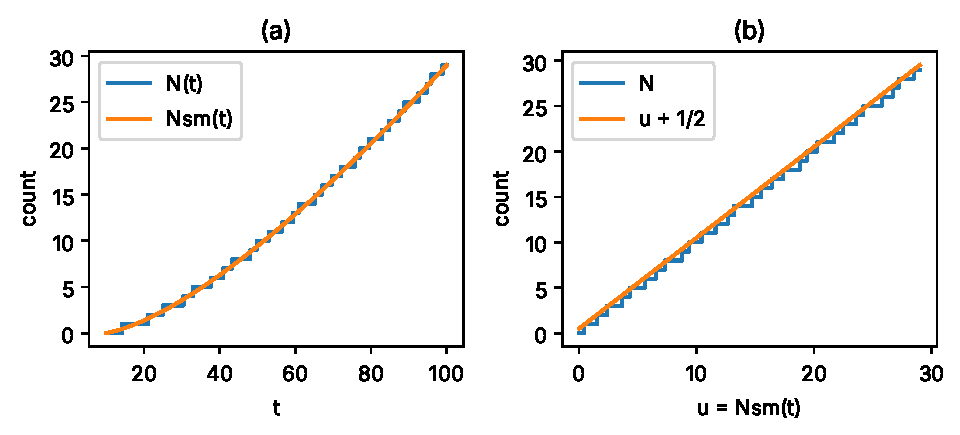
\includegraphics[width=0.85\linewidth]{figs/level-statistics_staircase.pdf}
\caption{Unfolding the zeros. (a) The staircase $N(t)$ (number of zeros up to height $t$) and the smooth counting function $\Nsm(t)$ of paper Eq.~(1), for $10\le t\le 100$; the steps get narrower as $t$ grows. (b) The same staircase drawn against the unfolded variable $u=\Nsm(t)$: now the steps have mean width one everywhere, and the straight line $N=u$ passes through the middle of the steps (because $\Nsm(s_n)=n-\tfrac12$ and $N(t_n)=n-\tfrac12$ by the midpoint convention).}
\label{fig:level-statistics-staircase}
\end{figure}

\begin{sample}{Unfolding the box: a perfect picket fence}
The levels of a particle in a box $[-L,L]$ with Dirichlet walls are the eigenvalues $E_k=(k\pi/2L)^2$, $k=1,2,\dots$ of $-y''=\lambda y$ (Chapter~\ref{ch:eigen}). Take $L=44.883$ (the paper's scale-1 box, running example RE3). Find $E_1$, $E_{500}$, the raw spacings at the bottom and near level 500, and the unfolded spacings.

\textbf{Step 1: raw levels.} $\pi/(2L)=\pi/89.766=0.0349976$, so $E_1=(0.0349976)^2=1.2248\times10^{-3}$ and $E_{500}=500^2E_1=306.2$.

\textbf{Step 2: raw spacings.} $E_{k+1}-E_k=\left[(k+1)^2-k^2\right]E_1=(2k+1)E_1$. At the bottom, $E_2-E_1=3E_1=3.674\times10^{-3}$; near level 500, $E_{501}-E_{500}=1001\,E_1=1.226$. The raw spacings grow linearly with $k$.

\textbf{Step 3: smooth counting function.} Level $k$ lies below $E$ when $k\pi/2L<\sqrt E$, that is $k<2L\sqrt E/\pi$. So away from the jumps the staircase is $N(E)=\lfloor 2L\sqrt{E}/\pi\rfloor$ (the floor function rounds down). At a level itself the midpoint convention gives $k-\tfrac12$ instead. Between levels $k$ and $k+1$ the quantity $2L\sqrt E/\pi$ runs from $k$ to $k+1$ while $N=k$, so the staircase lies on average half a step below it. The smooth function about which $N$ oscillates is therefore $\bar N(E)=2L\sqrt E/\pi-\tfrac12$, and $N-\bar N$ stays between $-\tfrac12$ and $+\tfrac12$.

\textbf{Step 4: unfold.} $u_k=\bar N(E_k)=\dfrac{2L}{\pi}\cdot\dfrac{k\pi}{2L}-\dfrac12=k-\dfrac12$, so $\delta_k=u_k-(k-\tfrac12)=0$ for every $k$.

\textbf{Answer:} \[\boxed{\Delta u_k=1\ \text{for every }k}\] Although the raw spacings differ by a factor $333.67$ between the bottom and level 500, the unfolded spectrum is an exact picket fence: zero variance, no fluctuation.
\end{sample}

\begin{sample}{Unfolding the first ten zeros}
Using paper Eq.~(1), unfold the first ten zeros (running example RE1) and list the unfolded spacings.

\textbf{Step 1: one value in full.} For $t_1=14.134725$: $t_1/2\pi=2.249611$, $\log 2.249611=0.810757$, so
$\Nsm(t_1)=2.249611\times0.810757-2.249611+0.875=1.823889-2.249611+0.875=0.449$.

\textbf{Step 2: all ten.} Repeating Step 1 (or running the listing below) gives Table~\ref{tab:level-statistics-re1}.

\textbf{Step 3: spacings and fluctuations.} Subtract consecutive $u_n$ for $\Delta u_n$, and subtract $n-\tfrac12$ for $\delta_n$.

\textbf{Step 4: mean spacing.} The nine spacings sum to $u_{10}-u_1=9.348-0.449=8.899$, so their mean is $0.989$, close to one as Eq.~\eqref{eq:level-statistics-meanone} promised.

\textbf{Answer:} \[\boxed{\Delta u_n = 1.121,\ 0.823,\ 1.278,\ 0.646,\ 1.276,\ 0.972,\ 0.729,\ 1.476,\ 0.578}\]
Notice two things. No spacing is small (the smallest is $0.578$), and long and short spacings tend to alternate. Both are features of the pattern you will learn to quantify.
\end{sample}

\begin{table}[htbp]\centering
\caption{Unfolding the first ten zeros (RE1) with paper Eq.~(1). $u_n=\Nsm(t_n)$, $\delta_n=u_n-(n-\tfrac12)$, $\Delta u_n=u_{n+1}-u_n$.}
\label{tab:level-statistics-re1}
\begin{tabular}{rcccc}
\toprule
$n$ & $t_n$ & $u_n$ & $\delta_n$ & $\Delta u_n$ \\
\midrule
1 & 14.134725 & 0.449 & $-0.051$ & 1.121\\
2 & 21.022040 & 1.570 & $+0.070$ & 0.823\\
3 & 25.010858 & 2.393 & $-0.107$ & 1.278\\
4 & 30.424876 & 3.671 & $+0.171$ & 0.646\\
5 & 32.935062 & 4.317 & $-0.183$ & 1.276\\
6 & 37.586178 & 5.593 & $+0.093$ & 0.972\\
7 & 40.918719 & 6.565 & $+0.065$ & 0.729\\
8 & 43.327073 & 7.294 & $-0.206$ & 1.476\\
9 & 48.005151 & 8.771 & $+0.271$ & 0.578\\
10 & 49.773832 & 9.348 & $-0.152$ & \\
\bottomrule
\end{tabular}
\end{table}

\begin{pycode}
import numpy as np, qmnt
t = qmnt.zeros(10)               # first ten zeros t_1..t_10
u = qmnt.Nsm(t)                  # unfolded levels u_n = Nsm(t_n)
n = np.arange(1, 11)
print(np.round(u, 3))
print(np.round(u - (n - 0.5), 3))   # fluctuations delta_n
print(np.round(np.diff(u), 3))      # unfolded spacings
\end{pycode}

How good is the local-gap shortcut of Eq.~\eqref{eq:level-statistics-localgap} here? The raw spacing is $t_2-t_1=6.887$; at the midpoint $\bar t=17.578$ the mean gap is $6.107$, so the shortcut gives $1.128$ instead of the exact $1.121$. The relative difference, $(1.121-1.128)/1.128=-0.0062$, is what Eq.~\eqref{eq:level-statistics-shortcuterr} predicts: with $\Delta^2=47.43$, $\bar t^{\,2}=309.0$ and $\log(\bar t/2\pi)=1.0288$, it gives $-47.43/(24\times309.0\times1.0288)=-0.0062$. Higher up the error shrinks rapidly, because $\Delta$ shrinks and $\bar t$ grows.

\begin{pitfall}
Unfolding with the wrong smooth function does not merely shift numbers: it changes the shape of every statistic. If $\bar N$ grows too fast in some region, spacings there are inflated and the histogram acquires a spurious tail. Always check that your unfolded spacings have mean one over each part of the spectrum you study, not just overall.
\end{pitfall}

\begin{checkpoint}
A spectrum has mean spacing $0.5$ in one region and $2$ in another. After correct unfolding, what is the mean spacing in each region?
\end{checkpoint}
\checkanswer{One in both regions. Unfolding divides out the local density, so every region has unit mean spacing; only the pattern of fluctuations about that mean remains.}

\begin{keyideas}
\item Unfolding $u_n=\bar N(E_n)$ with a smooth counting function $\bar N$ removes the changing density; unfolded spacings have mean one (Eq.~\eqref{eq:level-statistics-meanone}).
\item For the zeros, $\bar N=\Nsm$ of paper Eq.~(1), and the mean gap is $2\pi/\log(t/2\pi)$ (Eq.~\eqref{eq:level-statistics-gap}).
\item The fluctuation $\delta_n=u_n-(n-\tfrac12)$ equals the paper's $(t_n-s_n)/\gap_n$ to first order (Eq.~\eqref{eq:level-statistics-flucequiv}). ``Units of mean spacing'' means unfolded units.
\end{keyideas}

%=====================================================================
\section{The nearest-neighbor spacing distribution}\label{sec:level-statistics-spacing}
% DYK-BEGIN
\begin{didyouknow}{Wigner's Inspired Guess}
In 1956 Eugene Wigner proposed that spacings $s$ between neighboring energy levels of heavy nuclei follow $p(s)=\tfrac{\pi s}{2}e^{-\pi s^2/4}$, a formula derived from mere $2\times2$ random matrices. It vanishes at $s=0$, so levels repel each other. A companion formula from $2\times2$ complex Hermitian matrices, with $s^2$ in place of $s$, describes Riemann zero spacings remarkably well.
\end{didyouknow}
% DYK-END

Once a spectrum is unfolded, the simplest statistic is the distribution of the gaps between neighbors.

\textbf{Definition.} The \textbf{nearest-neighbor spacing distribution} is the probability density $p(s)$ such that, for a spacing chosen at random from a long unfolded spectrum,
\begin{equation}
\Pr\left(s<\Delta u\le s+\dd s\right)=p(s)\,\dd s .
\label{eq:level-statistics-pdef}
\end{equation}
Because it is a probability density on $s\ge0$ and because unfolding forces the mean spacing to be one, every spacing distribution in this chapter obeys two conditions:
\begin{equation}
\int_0^\infty p(s)\,\dd s=1,\qquad \int_0^\infty s\,p(s)\,\dd s=1 .
\label{eq:level-statistics-twoconditions}
\end{equation}
The first is normalization (Chapter~\ref{ch:probability}); the second is the unit mean. These two conditions will fix all the constants in the Wigner surmises. Keep in mind which laws are exact. The Poisson law will be derived exactly for independent levels, and the Wigner surmises exactly for $2\times2$ random matrices. For large random matrices, and for the zeros, the surmises are only close approximations to the true spacing distributions (see the box on large matrices in Sec.~\ref{sec:level-statistics-wigner}).

\textbf{Estimating $p(s)$ from data.} Given $K$ unfolded spacings, divide the $s$ axis into bins of width $b$. If $c_j$ spacings fall in bin $j$, the histogram estimate of $p$ at the center of that bin is
\begin{equation}
\hat p_j=\frac{c_j}{K\,b},
\label{eq:level-statistics-hist}
\end{equation}
the fraction of spacings in the bin divided by the bin width, so that $\sum_j\hat p_j\,b=1$, the discrete version of the first condition. This is what \texttt{density=True} does in a Matplotlib histogram, and it is how the bars of paper Fig.~2 are scaled.

Besides the mean, two summaries of $p(s)$ are useful: its variance $\int (s-1)^2p(s)\,\dd s=\int s^2p\,\dd s-1$, which measures how irregular the spacings are, and its behavior near $s=0$, which measures how often levels nearly collide. A picket fence has every spacing equal to one, so its variance is zero.

\begin{checkpoint}
Ten thousand unfolded spacings are binned with width $b=0.1$, and 1100 of them fall in the bin $0.9<s\le1.0$. What is the histogram estimate of $p$ in that bin?
\end{checkpoint}
\checkanswer{$\hat p=1100/(10000\times0.1)=1.1$. Note that a density can exceed one; only its integral must equal one.}

\begin{keyideas}
\item $p(s)\,\dd s$ is the probability that a random unfolded spacing lies in $[s,s+\dd s]$.
\item Every unfolded spacing density satisfies $\int p=1$ and $\int sp=1$ (Eq.~\eqref{eq:level-statistics-twoconditions}).
\item Histograms estimate $p$ by count$/(K\times$bin width$)$.
\end{keyideas}

%=====================================================================
\section{Uncorrelated levels: the Poisson law}\label{sec:level-statistics-poisson}

What would the spacings look like if levels knew nothing about each other? Model this by throwing $K$ points independently and uniformly onto an interval of length $K$ (we write $K$ because $N$ already denotes the counting function), so the mean density is one point per unit length (unfolded from the start).

\subsection{Derivation from the finite model}

Pick one of the points; call its position $y$, and suppose $y$ is not within distance $s$ of the right end. This costs nothing in the limit. A reference point chosen at random lies within $s$ of the right end with probability $s/K$ (the length of that strip divided by the total length), and for fixed $s$ this tends to zero as $K\to\infty$. Because all $K$ points were thrown independently, knowing where the reference point landed tells us nothing about the other $K-1$: each of them is still uniform on the whole interval. The nearest neighbor to the right is farther than $s$ exactly when none of the other $K-1$ points lands in the interval $(y,y+s]$.

\textbf{One other point.} Because it is uniform on a length $K$, it lands in an interval of length $s$ with probability $s/K$, and misses it with probability $1-s/K$.

\textbf{All other points.} They are independent, so the probabilities multiply (Chapter~\ref{ch:probability}):
\begin{equation}
Q_K(s)\equiv\Pr(\text{spacing}>s)=\left(1-\frac{s}{K}\right)^{K-1}.
\end{equation}

\textbf{The limit $K\to\infty$.} Take logarithms and use the Taylor series $\log(1-x)=-x-\tfrac{x^2}{2}-\tfrac{x^3}{3}-\cdots$, valid for $|x|<1$ (Chapter~\ref{ch:series}), with $x=s/K$:
\begin{align}
\log Q_K(s)&=(K-1)\log\left(1-\frac sK\right)\nonumber\\
&=(K-1)\left(-\frac sK-\frac{s^2}{2K^2}-\cdots\right)\nonumber\\
&=-s+\frac sK-\frac{(K-1)s^2}{2K^2}-\cdots .
\end{align}
Each term after $-s$ carries at least one factor $1/K$. There are infinitely many of them, so we bound their sum rather than treating them one at a time. For $0\le x\le\tfrac12$,
\begin{equation}
\left|\log(1-x)+x\right|=\frac{x^2}{2}+\frac{x^3}{3}+\cdots\le\frac{x^2}{2}\left(1+x+x^2+\cdots\right)=\frac{x^2}{2(1-x)}\le x^2 .
\end{equation}
The first inequality replaces each coefficient $1/j$ ($j\ge3$) by the larger $1/2$. The next step sums the geometric series (Chapter~\ref{ch:series}), and the last uses $1-x\ge\tfrac12$. Now write $\log Q_K(s)=(K-1)\left[\log(1-x)+x\right]-(K-1)x$ and note that $(K-1)x=s-s/K$. Then, for $K\ge2s$ (so that $x\le\tfrac12$),
\begin{equation}
\left|\log Q_K(s)+s\right|\le(K-1)x^2+\frac sK\le\frac{s^2}{K}+\frac sK\to0\qquad(K\to\infty).
\end{equation}
Hence $\log Q_K(s)\to-s$, and
\begin{equation}
Q(s)=e^{-s}.
\label{eq:level-statistics-survival}
\end{equation}

\textbf{From survival to density.} The probability that the spacing lies between $s$ and $s+\dd s$ is the probability that it exceeds $s$ minus the probability that it exceeds $s+\dd s$:
\begin{equation}
p(s)\,\dd s=Q(s)-Q(s+\dd s)=-\frac{\dd Q}{\dd s}\,\dd s
\quad\Longrightarrow\quad
\boxed{\;p_{\rm P}(s)=e^{-s}\;}
\label{eq:level-statistics-poisson}
\end{equation}
This is the exponential distribution that Chapter~\ref{ch:probability} introduced for gaps of a Poisson process, and the curve labeled ``Poisson'' in paper Fig.~2.

\subsection{Check of the two conditions, and the variance}

$\int_0^\infty e^{-s}\dd s=1$. By parts, $\int_0^\infty s e^{-s}\dd s=\left[-se^{-s}\right]_0^\infty+\int_0^\infty e^{-s}\dd s=0+1=1$. Again by parts, $\int_0^\infty s^2e^{-s}\dd s=\left[-s^2e^{-s}\right]_0^\infty+2\int_0^\infty se^{-s}\dd s=2$. So the variance is $2-1=1$: Poisson spacings are very irregular, with standard deviation equal to the mean.

\subsection{The most probable spacing is zero}

The density $e^{-s}$ is largest at $s=0$. In an uncorrelated spectrum, near-coincidences are the single most common kind of spacing. This is \textbf{clumping}: independence does not spread points out evenly, it produces clusters and voids. (Raindrops on a dry pavement show the same thing: some spots get hit twice before others are hit at all.)

\begin{pitfall}
``Random'' does not mean ``evenly spread.'' Many people, asked to draw random dots, space them too evenly. A truly uncorrelated pattern has more close pairs than any other kind of spacing. An evenly spread pattern is evidence of correlation (in this case repulsion), not of randomness.
\end{pitfall}

\begin{sample}{How rare are small and large gaps?}
For an unfolded spectrum, compare the probability that a spacing is below $0.1$, and the probability that it exceeds $2$, under the Poisson law and under the GUE surmise $p_{\rm GUE}(s)=\frac{32}{\pi^2}s^2e^{-4s^2/\pi}$ (derived in Sec.~\ref{sec:level-statistics-wigner}).

\textbf{Step 1: Poisson, small gaps.} $\Pr(s<0.1)=1-Q(0.1)=1-e^{-0.1}=0.0952$.

\textbf{Step 2: GUE, small gaps.} With $B=4/\pi$, expand $e^{-Bs^2}=1-Bs^2+\cdots$ and integrate term by term:
$\int_0^{0.1}s^2(1-Bs^2)\,\dd s=\frac{(0.1)^3}{3}-B\frac{(0.1)^5}{5}=3.3333\times10^{-4}-2.546\times10^{-6}$. The next term is about $10^{-8}$. Multiplying by $32/\pi^2=3.2423$ gives $\Pr(s<0.1)=1.073\times10^{-3}$.

\textbf{Step 3: ratio.} $0.0952/0.00107\approx89$: small gaps are about 89 times rarer under GUE.

\textbf{Step 4: large gaps, Poisson.} $\Pr(s>2)=Q(2)=e^{-2}=0.135$.

\textbf{Step 5: large gaps, GUE.} Write $A=32/\pi^2$ and $B=4/\pi$, and note that $A=2B^2$ (because $2\cdot16/\pi^2=32/\pi^2$). Then $\Pr(s>2)=A\int_2^\infty s\cdot se^{-Bs^2}\,\dd s$. Integrate by parts with $f=s$ and $\dd g=se^{-Bs^2}\dd s$, so $g=-e^{-Bs^2}/(2B)$:
\[
\int_2^\infty s^2e^{-Bs^2}\dd s=\left[-\frac{se^{-Bs^2}}{2B}\right]_2^\infty+\frac{1}{2B}\int_2^\infty e^{-Bs^2}\dd s=\frac{e^{-4B}}{B}+\frac{1}{2B}\int_2^\infty e^{-Bs^2}\dd s .
\]
In the last integral substitute $w=\sqrt B\,s$: it becomes $\frac{1}{\sqrt B}\int_{2\sqrt B}^\infty e^{-w^2}\dd w=\frac{\sqrt\pi}{2\sqrt B}\,\mathrm{erfc}(2\sqrt B)$, where $\mathrm{erfc}(z)=\frac{2}{\sqrt\pi}\int_z^\infty e^{-w^2}\dd w$ is the complementary error function, a tabulated function (\texttt{scipy.special.erfc}). Multiplying by $A=2B^2$:
\[
\Pr(s>2)=2Be^{-4B}+\frac{\sqrt{\pi B}}{2}\,\mathrm{erfc}(2\sqrt B)=\frac{8}{\pi}e^{-16/\pi}+\mathrm{erfc}\!\left(\frac{4}{\sqrt\pi}\right),
\]
using $\sqrt{\pi B}=2$. Numerically this is $0.0156+0.0014=0.017$, about 8 times rarer than Poisson.

\textbf{Answer:}
\[\boxed{\Pr(s<0.1):\ 0.0952\ \text{(Poisson)}\ \text{vs}\ 1.07\times10^{-3}\ \text{(GUE)};\quad \Pr(s>2):\ 0.135\ \text{vs}\ 0.017}\]
A repulsive spectrum suppresses both extremes: it is more regular than a Poisson one at both ends.
\end{sample}

\begin{keyideas}
\item Independent levels give $p_{\rm P}(s)=e^{-s}$ (Eq.~\eqref{eq:level-statistics-poisson}), derived from $(1-s/N)^{N-1}\to e^{-s}$.
\item Poisson spacings have mean 1, variance 1, and most probable value 0: uncorrelated levels clump.
\end{keyideas}

%=====================================================================
\section{Level repulsion and avoided crossings}\label{sec:level-statistics-repulsion}

Why would eigenvalues of a matrix avoid each other? The answer is already visible in $2\times2$ matrices.

\subsection{Eigenvalues of a real symmetric $2\times2$ matrix}

Take
\begin{equation}
H=\begin{pmatrix} a & b\\ b & d\end{pmatrix},\qquad a,b,d\ \text{real}.
\end{equation}
Its characteristic polynomial (Chapter~\ref{ch:eigen}) is
\begin{align}
\det(H-\lambda I)&=(a-\lambda)(d-\lambda)-b^2\nonumber\\
&=\lambda^2-(a+d)\lambda+ad-b^2 .
\end{align}
Setting it to zero and using the quadratic formula,
\begin{align}
\lambda_\pm&=\frac{(a+d)\pm\sqrt{(a+d)^2-4(ad-b^2)}}{2}\nonumber\\
&=\frac{a+d}{2}\pm\frac12\sqrt{a^2+2ad+d^2-4ad+4b^2}\nonumber\\
&=\frac{a+d}{2}\pm\frac12\sqrt{(a-d)^2+4b^2}.
\label{eq:level-statistics-2x2eig}
\end{align}
The spacing is therefore
\begin{equation}
\lambda_+-\lambda_-=\sqrt{(a-d)^2+4b^2}.
\label{eq:level-statistics-2x2gap}
\end{equation}
The two eigenvalues coincide only if $(a-d)^2+4b^2=0$, and since both terms are squares of real numbers this requires \emph{two} conditions at once: $a=d$ and $b=0$.

\subsection{Avoided crossings}

Let the matrix depend on a control parameter $\tau$ (think of a field strength you are turning up; we avoid $\lambda$, which denotes the eigenvalues), with a fixed coupling $g$:
\begin{equation}
H(\tau)=\begin{pmatrix}\tau & g\\ g & -\tau\end{pmatrix}.
\end{equation}
By Eq.~\eqref{eq:level-statistics-2x2eig} with $a=\tau$, $d=-\tau$, $b=g$, the levels are $\pm\sqrt{\tau^2+g^2}$. Without coupling ($g=0$) the levels $\pm\tau$ cross at $\tau=0$. With any nonzero coupling they never meet: the smallest separation is $2|g|$, reached at $\tau=0$ (Fig.~\ref{fig:level-statistics-avoided}). This is an \textbf{avoided crossing}. Mechanically, it is like two pendulums joined by a weak spring: when their natural frequencies are tuned past each other, the frequencies of the coupled system approach and then turn away.

\begin{figure}[htbp]\centering
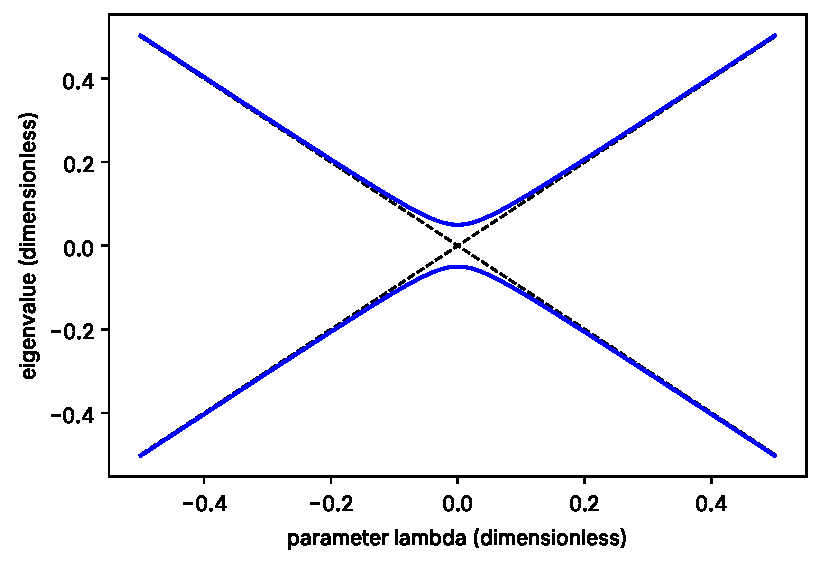
\includegraphics[width=0.85\linewidth]{figs/level-statistics_avoided.pdf}
\caption{Eigenvalues of $H(\tau)=\begin{pmatrix}\tau&g\\g&-\tau\end{pmatrix}$ as functions of the dimensionless control parameter $\tau$. Dashed: $g=0$, the levels $\pm\tau$ cross. Solid: $g=0.05$, the levels $\pm\sqrt{\tau^2+g^2}$ never meet; their minimum separation is $2g=0.1$ at $\tau=0$.}
\label{fig:level-statistics-avoided}
\end{figure}

\begin{sample}{Eigenvalues, spacing, and an avoided crossing}
(a) Find the eigenvalues and spacing of $H=\begin{pmatrix}1&0.3\\0.3&1.2\end{pmatrix}$. (b) For $H(\tau)$ above with $g=0.05$, find the spacing at $\tau=0$ and $\tau=0.2$, and compare with the uncoupled spacing $2|\tau|$.

\textbf{Step 1:} In (a), $a=1$, $d=1.2$, $b=0.3$. The center is $(a+d)/2=1.1$.

\textbf{Step 2:} Spacing from Eq.~\eqref{eq:level-statistics-2x2gap}: $\sqrt{(1-1.2)^2+4(0.3)^2}=\sqrt{0.04+0.36}=\sqrt{0.40}=0.6325$.

\textbf{Step 3:} Eigenvalues $1.1\pm0.3162$, i.e.\ $0.7838$ and $1.4162$. Check: their sum $2.2$ equals the trace $a+d$, and their product $1.1^2-0.3162^2=1.11$ equals $\det H=1.2-0.09=1.11$.

\textbf{Step 4:} In (b), the spacing is $2\sqrt{\tau^2+g^2}$. At $\tau=0$: $2g=0.1$. At $\tau=0.2$: $2\sqrt{0.04+0.0025}=0.4123$, compared with $0.4$ without coupling.

\textbf{Answer:} \[\boxed{\lambda_\pm=0.7838,\ 1.4162;\ \text{spacing }0.6325;\ \text{avoided crossing: }0.1\ (\tau=0),\ 0.4123\ (\tau=0.2)}\]
Far from the crossing the coupling hardly matters; near it, it dominates.
\end{sample}

\subsection{Counting conditions}

Here is the key idea behind level repulsion. A real symmetric $2\times2$ matrix has three free numbers $(a,b,d)$, but a degeneracy needs two of them to be tuned (the combinations $a-d$ and $b$). If the matrix is ``generic'' (its entries are random and smoothly distributed), hitting two conditions by accident is very unlikely, much less likely than hitting one. For a complex Hermitian matrix the off-diagonal entry $b$ is complex, with a real and an imaginary part, so a degeneracy needs \emph{three} conditions. In the next section we turn this counting into exact formulas.

By contrast, consider a \emph{diagonal} random matrix ($b=0$ always). Then the spacing is $|a-d|$, a single condition, and nothing prevents near-coincidences: the eigenvalues are just two independent numbers. Repulsion is caused by the off-diagonal mixing.

\begin{checkpoint}
Two levels belong to two completely separate systems (for example, two boxes far apart), so their Hamiltonian is block diagonal and no matrix element connects them. Do these two levels repel?
\end{checkpoint}
\checkanswer{No. Without a coupling matrix element there is no avoided crossing; their spacing behaves like the difference of two independent numbers. When the spectra of unrelated systems are superposed, close pairs are therefore no longer suppressed. With many superposed spectra the statistics approach Poisson; this is a known result that we state without proof (see \cite{mehta}).}

\begin{keyideas}
\item For a real symmetric $2\times2$ matrix, the spacing is $\sqrt{(a-d)^2+4b^2}$ (Eq.~\eqref{eq:level-statistics-2x2gap}); a degeneracy needs two conditions.
\item Coupling turns crossings into avoided crossings with minimum gap $2|g|$.
\item Repulsion comes from off-diagonal mixing; levels of uncoupled systems do not repel.
\end{keyideas}

%=====================================================================
\section{Random $2\times2$ matrices and the Wigner surmises}\label{sec:level-statistics-wigner}

\subsection{A toolkit of Gaussian integrals}

We will need the integrals
\begin{equation}
I_k(B)=\int_0^\infty s^k e^{-Bs^2}\,\dd s,\qquad B>0,\quad k=0,1,2,\dots
\label{eq:level-statistics-Ik}
\end{equation}

\textbf{$I_0$.} Recall from Chapter~\ref{ch:probability} that the Gaussian density integrates to one; equivalently $G\equiv\int_{-\infty}^{\infty}e^{-Bx^2}\dd x=\sqrt{\pi/B}$. For completeness, here is why. Write $G^2$ as a product of two copies, one in $x$ and one in $y$. As Riemann sums, $\left(\sum_i e^{-Bx_i^2}\Delta x\right)\left(\sum_j e^{-By_j^2}\Delta y\right)=\sum_{i,j}e^{-B(x_i^2+y_j^2)}\Delta x\,\Delta y$, a sum over little squares tiling the plane. The integrand depends only on the distance $r=\sqrt{x^2+y^2}$ from the origin, so group the squares into thin rings of radius $r$ and width $\dd r$, each of area $2\pi r\,\dd r$:
\begin{equation}
G^2=\int_0^\infty e^{-Br^2}\,2\pi r\,\dd r=2\pi\left[-\frac{e^{-Br^2}}{2B}\right]_0^\infty=\frac{\pi}{B}.
\end{equation}
So $G=\sqrt{\pi/B}$, and because the integrand is even, $I_0=\tfrac12\sqrt{\pi/B}$.

\textbf{$I_1$.} Substituting directly, $I_1=\left[-\dfrac{e^{-Bs^2}}{2B}\right]_0^\infty=\dfrac{1}{2B}$.

\textbf{Recursion.} For $k\ge0$, integrate $I_{k+2}=\int_0^\infty s^{k+1}\cdot s e^{-Bs^2}\dd s$ by parts with $f=s^{k+1}$ and $\dd g=se^{-Bs^2}\dd s$, so $g=-e^{-Bs^2}/(2B)$:
\begin{equation}
I_{k+2}=\left[-\frac{s^{k+1}e^{-Bs^2}}{2B}\right]_0^\infty+\frac{k+1}{2B}\int_0^\infty s^ke^{-Bs^2}\dd s=\frac{k+1}{2B}I_k .
\end{equation}
The boundary term vanishes at $s=0$ because $s^{k+1}=0$ there, and at infinity because the exponential decays faster than any power grows. Hence
\begin{equation}
I_2=\frac{\sqrt\pi}{4B^{3/2}},\qquad I_3=\frac{1}{2B^2},\qquad I_4=\frac{3\sqrt\pi}{8B^{5/2}}.
\label{eq:level-statistics-I234}
\end{equation}

\subsection{The real symmetric case: a spacing density proportional to $s$}

Any real symmetric $2\times2$ matrix can be written as
\begin{equation}
H=\begin{pmatrix} c+\tfrac x2 & \tfrac y2\\[2pt] \tfrac y2 & c-\tfrac x2\end{pmatrix},
\qquad c=\frac{a+d}{2},\ x=a-d,\ y=2b .
\label{eq:level-statistics-param}
\end{equation}
By Eq.~\eqref{eq:level-statistics-2x2gap}, its spacing is
\begin{equation}
s=\sqrt{x^2+y^2},
\end{equation}
the distance of the point $(x,y)$ from the origin of a plane. The center $c$ shifts both levels together and does not affect $s$.

Now make the matrix random: let $x$ and $y$ be independent Gaussian random variables with mean zero and the same variance $\sigma^2$. Independence means the probability of landing in a small rectangle $\dd x\,\dd y$ is the product of the two one-dimensional probabilities:
\begin{equation}
\frac{1}{\sqrt{2\pi}\sigma}e^{-x^2/2\sigma^2}\dd x\cdot\frac{1}{\sqrt{2\pi}\sigma}e^{-y^2/2\sigma^2}\dd y
=\frac{1}{2\pi\sigma^2}e^{-(x^2+y^2)/2\sigma^2}\,\dd x\,\dd y .
\end{equation}
This joint density depends only on the distance $s$ from the origin. So the probability that the spacing lies between $s$ and $s+\dd s$ is the density on the ring of radius $s$ times the area $2\pi s\,\dd s$ of that ring:
\begin{equation}
p(s)\,\dd s=\frac{1}{2\pi\sigma^2}e^{-s^2/2\sigma^2}\cdot 2\pi s\,\dd s
\quad\Longrightarrow\quad
p(s)=\frac{s}{\sigma^2}\,e^{-s^2/2\sigma^2}.
\label{eq:level-statistics-rayleigh}
\end{equation}
The factor $s$ is the circumference of the ring. That is level repulsion in its purest form: small spacings need $(x,y)$ to fall in a small disk around the origin, and a small disk has tiny area.

\textbf{Normalization check.} With $B=1/(2\sigma^2)$, $\int p\,\dd s=\frac{1}{\sigma^2}I_1=\frac{1}{\sigma^2}\cdot\frac{1}{2B}=\frac{2\sigma^2}{2\sigma^2}=1$.

\textbf{Mean spacing.} $\langle s\rangle=\frac{1}{\sigma^2}I_2=\frac{1}{\sigma^2}\cdot\frac{\sqrt\pi\,(2\sigma^2)^{3/2}}{4}=\frac{\sqrt\pi\,2\sqrt2\,\sigma^3}{4\sigma^2}=\sigma\sqrt{\frac{\pi}{2}}$.

\subsection{Unfolding the $2\times2$ ensemble: rescaling a density}

A $2\times2$ matrix has only one spacing, so ``unfolding'' means dividing by the ensemble mean: $s'=s/\langle s\rangle$. How does a density change under a rescaling $s'=s/\ell$? The event ``$s'$ in $[s',s'+\dd s']$'' is the same event as ``$s$ in $[\ell s',\ell s'+\ell\,\dd s']$'', so $p'(s')\,\dd s'=p(\ell s')\,\ell\,\dd s'$, i.e.
\begin{equation}
p'(s')=\ell\,p(\ell s').
\label{eq:level-statistics-rescale}
\end{equation}
With $\ell=\langle s\rangle=\sigma\sqrt{\pi/2}$ and Eq.~\eqref{eq:level-statistics-rayleigh}:
\begin{align}
p'(s')&=\ell\cdot\frac{\ell s'}{\sigma^2}e^{-\ell^2s'^2/2\sigma^2}\nonumber\\
&=\frac{\ell^2}{\sigma^2}\,s'\,e^{-(\ell^2/2\sigma^2)s'^2}\nonumber\\
&=\frac{\pi}{2}\,s'\,e^{-\pi s'^2/4}\qquad\text{(using }\ell^2/\sigma^2=\pi/2).
\end{align}
The variance $\sigma^2$ has dropped out completely. Dropping the prime:
\begin{equation}
\boxed{\;p_{\rm GOE}(s)=\frac{\pi}{2}\,s\,e^{-\pi s^2/4}\;}
\label{eq:level-statistics-goe}
\end{equation}
This is the \textbf{Wigner surmise} for real symmetric matrices.

\textbf{Cross-check by the two conditions.} Suppose we only knew that $p(s)=As\,e^{-Bs^2}$. Then Eq.~\eqref{eq:level-statistics-twoconditions} gives $AI_1=A/(2B)=1$, so $A=2B$, and $AI_2=2B\sqrt\pi/(4B^{3/2})=\sqrt\pi/(2\sqrt B)=1$, so $\sqrt B=\sqrt\pi/2$, $B=\pi/4$, $A=\pi/2$, the same result. The two conditions determine $A$ and $B$ uniquely.

\subsection{The complex Hermitian case: a spacing density proportional to $s^2$}

A complex Hermitian $2\times2$ matrix (Chapter~\ref{ch:eigen}) has real diagonal entries and complex conjugate off-diagonal entries. Write it as
\begin{equation}
H=\begin{pmatrix} c+\tfrac x2 & \tfrac{y-\ii z}{2}\\[2pt] \tfrac{y+\ii z}{2} & c-\tfrac x2\end{pmatrix},\qquad x,y,z,c\ \text{real}.
\label{eq:level-statistics-paramC}
\end{equation}
Its characteristic polynomial is
\begin{align}
\det(H-\lambda I)&=\left(c-\lambda+\tfrac x2\right)\left(c-\lambda-\tfrac x2\right)-\frac{(y-\ii z)(y+\ii z)}{4}\nonumber\\
&=(c-\lambda)^2-\frac{x^2}{4}-\frac{y^2+z^2}{4},
\end{align}
using $(y-\ii z)(y+\ii z)=y^2+z^2$ (Chapter~\ref{ch:complex}). Setting it to zero, $\lambda=c\pm\tfrac12\sqrt{x^2+y^2+z^2}$, so the spacing is
\begin{equation}
s=\sqrt{x^2+y^2+z^2},
\end{equation}
the length of the vector $(x,y,z)$ in ordinary three-dimensional space. A degeneracy needs three conditions, $x=y=z=0$.

Let $x,y,z$ be independent Gaussians with mean zero and variance $\sigma^2$. The joint density is $(2\pi\sigma^2)^{-3/2}e^{-(x^2+y^2+z^2)/2\sigma^2}$, constant on spheres. A thin spherical shell of radius $s$ and thickness $\dd s$ has volume $4\pi s^2\,\dd s$, so
\begin{equation}
p(s)=\frac{4\pi s^2}{(2\pi\sigma^2)^{3/2}}e^{-s^2/2\sigma^2}=\sqrt{\frac{2}{\pi}}\,\frac{s^2}{\sigma^3}\,e^{-s^2/2\sigma^2},
\label{eq:level-statistics-maxwell}
\end{equation}
where $4\pi/(2\pi)^{3/2}=2/\sqrt{2\pi}=\sqrt{2/\pi}$. (Physicists know this shape as the Maxwell speed distribution, for the same geometric reason.)

\textbf{Rescaling to unit mean.} By Eq.~\eqref{eq:level-statistics-rescale}, rescaling a density of the form $s^2e^{-Bs^2}$ produces another density of the same form, $As^2e^{-B's^2}$. So the unfolded density is $As^2e^{-Bs^2}$ with $A$ and $B$ fixed by the two conditions:
\begin{align}
\int_0^\infty As^2e^{-Bs^2}\dd s&=AI_2=\frac{A\sqrt\pi}{4B^{3/2}}=1, \label{eq:level-statistics-c1}\\
\int_0^\infty As^3e^{-Bs^2}\dd s&=AI_3=\frac{A}{2B^2}=1 .\label{eq:level-statistics-c2}
\end{align}
From Eq.~\eqref{eq:level-statistics-c2}, $A=2B^2$. Substituting into Eq.~\eqref{eq:level-statistics-c1}:
\begin{equation}
\frac{2B^2\sqrt\pi}{4B^{3/2}}=\frac{\sqrt\pi}{2}B^{1/2}=1
\quad\Longrightarrow\quad B^{1/2}=\frac{2}{\sqrt\pi}
\quad\Longrightarrow\quad B=\frac4\pi .
\end{equation}
Then $A=2B^2=2\cdot\dfrac{16}{\pi^2}=\dfrac{32}{\pi^2}$. Therefore
\begin{equation}
\boxed{\;p_{\rm GUE}(s)=\frac{32}{\pi^2}\,s^2\,e^{-4s^2/\pi}\;}
\label{eq:level-statistics-gue}
\end{equation}
This is exactly the curve in the caption of paper Fig.~2. Figure~\ref{fig:level-statistics-surmises} compares it with the GOE surmise and the Poisson law.

\subsection{Why these ensembles, and their names}

You may object that we \emph{chose} $x$ and $y$ (or $x,y,z$) to have equal variances. Here is the natural choice that produces it. Let the entries $a,d$ of a real symmetric matrix be independent Gaussians of variance $\sigma_0^2$, and let $b$ have variance $\sigma_0^2/2$. Then the joint density is proportional to
\begin{equation}
e^{-a^2/2\sigma_0^2}\,e^{-d^2/2\sigma_0^2}\,e^{-b^2/\sigma_0^2}=e^{-(a^2+d^2+2b^2)/2\sigma_0^2}=e^{-\mathrm{tr}(H^2)/2\sigma_0^2},
\end{equation}
because the \textbf{trace} (sum of diagonal entries) of $H^2$ is $a^2+b^2+b^2+d^2$. (Recall the matrix product from Chapter~\ref{ch:linear-algebra}: $(XY)_{ik}=\sum_jX_{ij}Y_{jk}$; for $H^2$ the diagonal entries are $a^2+b^2$ and $b^2+d^2$. A rotation of the plane is a real matrix $O$ with $O^\top O=I$, and $OHO^\top$ is the same linear map written in the rotated basis, Chapter~\ref{ch:linear-algebra}.) The trace has the property $\mathrm{tr}(XY)=\sum_i\sum_jX_{ij}Y_{ji}=\sum_j\sum_iY_{ji}X_{ij}=\mathrm{tr}(YX)$, so for any rotation $O$ (with $O^\top O=I$), $\mathrm{tr}\big((OHO^\top)^2\big)=\mathrm{tr}(OH^2O^\top)=\mathrm{tr}(H^2O^\top O)=\mathrm{tr}(H^2)$. Probabilities are densities times volumes, so one more fact is needed: the volume element $\dd a\,\dd b\,\dd d$ must also be unchanged. It is. The map $H\to OHO^\top$ changes the triple $(a,\sqrt2\,b,d)$ linearly (each new entry is a fixed combination of the old ones), and it preserves $a^2+2b^2+d^2=\mathrm{tr}(H^2)$, the squared length of that triple in a three-dimensional space. A linear map that preserves all lengths is a rotation or a reflection, and these preserve volumes. The ensemble therefore has no preferred basis: rotating every matrix leaves the probabilities unchanged. It is called the \textbf{Gaussian Orthogonal Ensemble (GOE)}.

Now convert to the variables of Eq.~\eqref{eq:level-statistics-param}. Since $a=c+x/2$ and $d=c-x/2$,
\begin{equation}
a^2+d^2=\left(c+\tfrac x2\right)^2+\left(c-\tfrac x2\right)^2=2c^2+\tfrac{x^2}{2},
\end{equation}
so the density in $(c,x)$ is proportional to $e^{-c^2/\sigma_0^2}\,e^{-x^2/4\sigma_0^2}$. (The change of variables is the linear map $a=c+\tfrac12x$, $d=c-\tfrac12x$, with matrix $J=\begin{pmatrix}1&\tfrac12\\1&-\tfrac12\end{pmatrix}$. A linear map with matrix $J$ sends a small rectangle of area $\dd c\,\dd x$ to a parallelogram of area $|\det J|\,\dd c\,\dd x$; this is the meaning of the $2\times2$ determinant as an area factor (Chapter~\ref{ch:linear-algebra}). A probability is a density times an area, so a density $f(a,d)$ becomes $f\,|\det J|$ when expressed in $(c,x)$. Here $\det J=1\cdot(-\tfrac12)-\tfrac12\cdot1=-1$, so $|\det J|=1$, and the density only needs re-expressing in the new variables.) The density factorizes, so $x$ is a Gaussian of variance $2\sigma_0^2$, independent of $c$. And $y=2b$ has variance $4\cdot\sigma_0^2/2=2\sigma_0^2$ (scaling rule $\mathrm{Var}(kX)=k^2\mathrm{Var}(X)$, Chapter~\ref{ch:probability}). So $x$ and $y$ are independent with equal variance $\sigma^2=2\sigma_0^2$, exactly our assumption.

\textbf{The complex case.} Now let $b$ denote the lower-left entry $(y+\ii z)/2$ of Eq.~\eqref{eq:level-statistics-paramC}. It is complex, $b=b_r+\ii b_i$, with $b_r,b_i$ independent Gaussians each of variance $\sigma_0^2/2$, and the upper-right entry is its conjugate $b_r-\ii b_i$. Comparing with Eq.~\eqref{eq:level-statistics-paramC}, $y=2b_r$ and $z=2b_i$, so each has variance $4\cdot\sigma_0^2/2=2\sigma_0^2$. The variable $x=a-d$ has variance $2\sigma_0^2$ and is independent of $c$, exactly as above. Finally $x$, $y$, $z$ are independent of each other because they are built separately from the independent numbers $(a,d)$, $b_r$ and $b_i$. So again all three components have the common variance $\sigma^2=2\sigma_0^2$. The joint density is proportional to
\[
e^{-(a^2+d^2)/2\sigma_0^2}\,e^{-(b_r^2+b_i^2)/\sigma_0^2}=e^{-(a^2+d^2+2|b|^2)/2\sigma_0^2}=e^{-\mathrm{tr}(H^2)/2\sigma_0^2},
\]
because the diagonal entries of $H^2$ are now $a^2+|b|^2$ and $|b|^2+d^2$. This is the \textbf{Gaussian Unitary Ensemble (GUE)}. Its density is unchanged under unitary changes of basis $H\to UHU^\dagger$ with $U^\dagger U=I$, by the same trace argument with $O^\top$ replaced by $U^\dagger$ (Problem 5 asks you to write out the trace step; the corresponding statement about volumes for complex entries we take on trust from \cite{mehta}).

Some physics background, which we state rather than derive. A Hamiltonian is the Hermitian matrix or operator whose eigenvalues are the energy levels of a quantum system (Chapter~\ref{ch:schrodinger} develops this). Time reversal means running the motion backward; for a wavefunction it amounts to complex conjugation. Real symmetric Hamiltonians arise for systems that are invariant under time reversal (no magnetic field, for instance), and complex Hermitian ones for systems where time-reversal symmetry is broken \cite{mehta}. The exponent of $s$ near zero is called the \textbf{Dyson index} $\beta$: $\beta=1$ for GOE, $\beta=2$ for GUE, and $\beta=4$ for a third (``symplectic'') ensemble treated in Problem 11. Poisson corresponds to $\beta=0$. The rule behind all of them is the counting of Sec.~\ref{sec:level-statistics-repulsion}: if a degeneracy needs $D$ independent conditions, then $p(s)\propto s^{D-1}$ near zero, with $D=2$ (GOE), $3$ (GUE), $5$ (symplectic). The first two follow from the counting above: one condition from the diagonal ($a=d$) plus one (real $b$) or two (complex $b$) from the off-diagonal entry. The symplectic value we quote rather than derive: in that ensemble the off-diagonal element of the $2\times2$ (quaternion) matrix has four real components, so a degeneracy needs $1+4=5$ conditions \cite{mehta}.

\begin{figure}[htbp]\centering
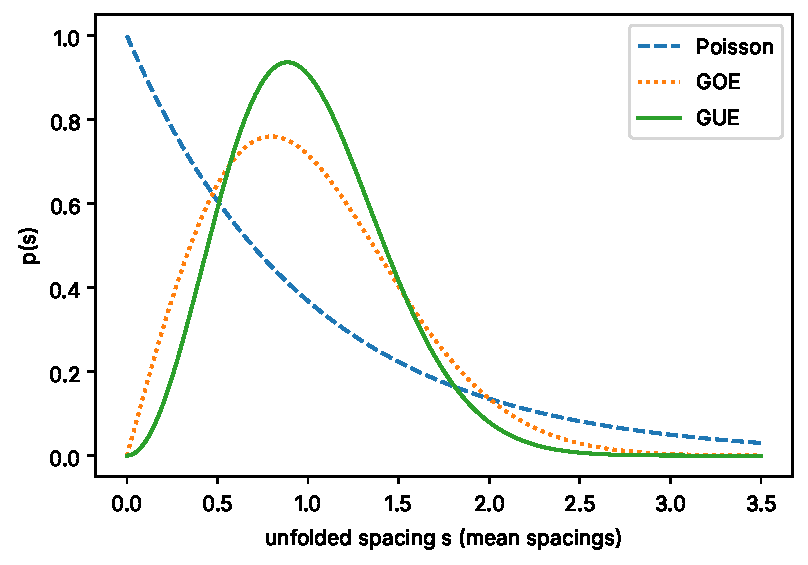
\includegraphics[width=0.85\linewidth]{figs/level-statistics_surmises.pdf}
\caption{The three reference spacing distributions for unfolded spectra (unit mean spacing): Poisson $e^{-s}$, GOE Wigner surmise $\frac{\pi}{2}se^{-\pi s^2/4}$, and GUE Wigner surmise $\frac{32}{\pi^2}s^2e^{-4s^2/\pi}$. The random-matrix laws vanish at $s=0$ (linearly for GOE, quadratically for GUE) and are much narrower than Poisson.}
\label{fig:level-statistics-surmises}
\end{figure}

\begin{sample}{Shape of the three distributions}
Find the most probable spacing and the variance for the Poisson, GOE and GUE distributions.

\textbf{Step 1: Poisson.} $e^{-s}$ is decreasing, so the most probable spacing is $0$; the variance is $1$ (Sec.~\ref{sec:level-statistics-poisson}).

\textbf{Step 2: GOE mode.} $\frac{\dd}{\dd s}\left(se^{-\pi s^2/4}\right)=e^{-\pi s^2/4}\left(1-\frac{\pi s^2}{2}\right)=0$ gives $s=\sqrt{2/\pi}=0.798$.

\textbf{Step 3: GUE mode.} $\frac{\dd}{\dd s}\left(s^2e^{-4s^2/\pi}\right)=e^{-4s^2/\pi}\left(2s-\frac{8s^3}{\pi}\right)=0$ gives $s^2=\pi/4$, $s=0.886$.

\textbf{Step 4: GOE variance.} $\langle s^2\rangle=\frac\pi2 I_3(\pi/4)=\frac\pi2\cdot\frac{1}{2(\pi/4)^2}=\frac\pi2\cdot\frac{8}{\pi^2}=\frac4\pi$, so the variance is $\frac4\pi-1=0.273$.

\textbf{Step 5: GUE variance.} $\langle s^2\rangle=\frac{32}{\pi^2}I_4(4/\pi)=\frac{32}{\pi^2}\cdot\frac{3\sqrt\pi}{8(4/\pi)^{5/2}}$. Since $(4/\pi)^{5/2}=32/\pi^{5/2}$, this is $\frac{32}{\pi^2}\cdot\frac{3\sqrt\pi\,\pi^{5/2}}{256}=\frac{3\pi^3}{8\pi^2}=\frac{3\pi}{8}$, so the variance is $\frac{3\pi}8-1=0.178$ (standard deviation $0.422$).

\textbf{Answer:}
\[\boxed{\text{mode: }0,\ 0.798,\ 0.886;\qquad \text{variance: }1,\ 0.273,\ 0.178\quad(\text{Poisson, GOE, GUE})}\]
Stronger repulsion means a more regular spectrum: GUE spacings are the least spread out of the three.
\end{sample}

\begin{sample}{The small-spacing laws}
Find $\Pr(s<\varepsilon)$ for small $\varepsilon$ under each law, and evaluate at $\varepsilon=0.1$.

\textbf{Step 1: Poisson.} $1-e^{-\varepsilon}\approx\varepsilon$ for small $\varepsilon$ (first-order Taylor). At $\varepsilon=0.1$: exact $0.0952$.

\textbf{Step 2: GOE, exact.} $\int_0^\varepsilon\frac\pi2se^{-\pi s^2/4}\dd s=\left[-e^{-\pi s^2/4}\right]_0^\varepsilon=1-e^{-\pi\varepsilon^2/4}\approx\frac\pi4\varepsilon^2$. At $\varepsilon=0.1$: exact $0.00782$, approximation $0.00785$.

\textbf{Step 3: GUE.} For small $s$, $e^{-4s^2/\pi}\approx1$, so $\int_0^\varepsilon\frac{32}{\pi^2}s^2\dd s=\frac{32}{3\pi^2}\varepsilon^3=1.081\varepsilon^3$. At $\varepsilon=0.1$: $1.081\times10^{-3}$, against the exact $1.073\times10^{-3}$ found earlier.

\textbf{Answer:}
\[\boxed{\Pr(s<\varepsilon)\approx\varepsilon\ (\text{Poisson}),\quad \tfrac\pi4\varepsilon^2\ (\text{GOE}),\quad \tfrac{32}{3\pi^2}\varepsilon^3\ (\text{GUE})}\]
Halving $\varepsilon$ halves the Poisson probability, quarters the GOE one, and divides the GUE one by eight. This is the most sensitive fingerprint of the symmetry class.
\end{sample}

\begin{pycode}
import numpy as np
rng = np.random.default_rng(0)        # fixed seed: reproducible
n = 200000                            # number of random 2x2 matrices
x, y, z = rng.normal(size=(3, n))     # independent N(0,1) numbers
s_real = np.hypot(x, y)               # GOE-type: s = sqrt(x^2 + y^2)
s_cplx = np.sqrt(x**2 + y**2 + z**2)  # GUE-type: s = |(x, y, z)|
for s in (s_real, s_cplx):
    s = s / s.mean()                  # unfold: unit mean spacing
    print(np.mean(s < 0.1), np.mean(s**2))
\end{pycode}
With this seed the printed small-gap fractions agree with the exact values $0.00782$ (GOE) and $1.07\times10^{-3}$ (GUE) of the sample problems to within three binomial standard errors. Here the standard error is $\sqrt{p(1-p)/n}$ with $n=2\times10^5$, about $2\times10^{-4}$ for GOE and $7\times10^{-5}$ for GUE (Chapter~\ref{ch:probability}). The values of $\langle s^2\rangle$ agree with $4/\pi$ and $3\pi/8$ to within $0.01$. Figure~\ref{fig:level-statistics-2x2sim} shows the histograms.

\begin{figure}[htbp]\centering
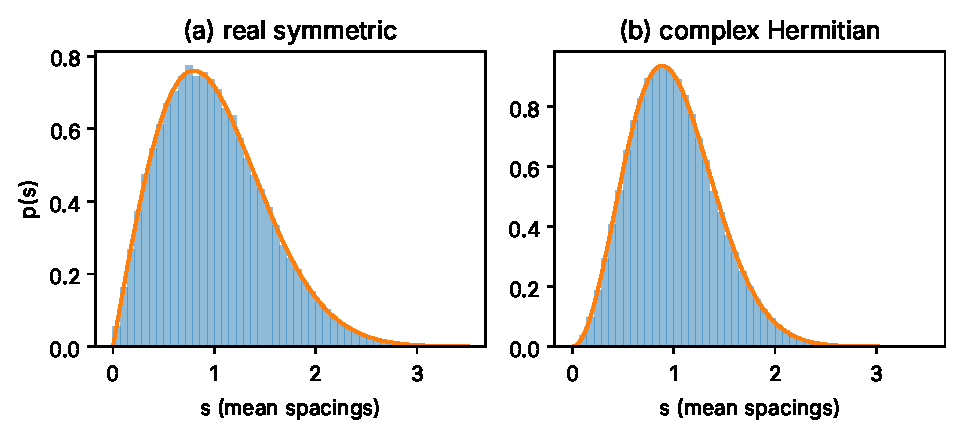
\includegraphics[width=0.85\linewidth]{figs/level-statistics_2x2sim.pdf}
\caption{Spacings of $2\times10^5$ random $2\times2$ matrices, each rescaled by the sample mean spacing. (a) Real symmetric matrices of the form of Eq.~\eqref{eq:level-statistics-param} with independent Gaussian $x,y$: the histogram follows the GOE surmise. (b) Complex Hermitian matrices of the form of Eq.~\eqref{eq:level-statistics-paramC}: the histogram follows the GUE surmise. Spacings are dimensionless (units of mean spacing).}
\label{fig:level-statistics-2x2sim}
\end{figure}

\begin{beyond}
\textbf{Large matrices.} The surmises are exact for $2\times2$ Gaussian matrices (proved above). For $N\times N$ GOE or GUE matrices with $N\to\infty$, the exact spacing distribution in the middle of the spectrum (after unfolding) is a more complicated function, found by Gaudin and Mehta and expressed through objects beyond this book. Numerically it is very close to the corresponding surmise, which is why the surmise is the standard benchmark, as in paper Fig.~2. Derivations are in \cite{mehta}. We take the closeness on trust.
\end{beyond}

\begin{checkpoint}
Why does the GUE density start like $s^2$ while the GOE density starts like $s$?
\end{checkpoint}
\checkanswer{A GUE degeneracy needs three real conditions ($x=y=z=0$), a GOE one only two. The probability of a spacing below $s$ is the probability of landing in a ball of radius $s$ around the origin: area $\propto s^2$ in 2D, volume $\propto s^3$ in 3D. Differentiating gives densities $\propto s$ and $\propto s^2$.}

\begin{keyideas}
\item Spacing of a $2\times2$ matrix $=$ length of a Gaussian vector: 2 components (real symmetric) or 3 (complex Hermitian).
\item Geometry (ring circumference $2\pi s$, shell area $4\pi s^2$) gives $p\propto s\,e^{-Bs^2}$ and $p\propto s^2e^{-Bs^2}$; the two conditions of Eq.~\eqref{eq:level-statistics-twoconditions} give $p_{\rm GOE}=\frac\pi2se^{-\pi s^2/4}$ and $p_{\rm GUE}=\frac{32}{\pi^2}s^2e^{-4s^2/\pi}$.
\item The Dyson index $\beta$ (0, 1, 2, 4) controls small-spacing behavior $\Pr(s<\varepsilon)\propto\varepsilon^{\beta+1}$.
\end{keyideas}

%=====================================================================
\section{Beyond nearest neighbors: pair correlation and Montgomery's discovery}\label{sec:level-statistics-pair}
% DYK-BEGIN
\begin{didyouknow}{Zeros at Dizzying Heights}
Starting in the 1980s, Andrew Odlyzko at Bell Labs computed huge batches of zeta zeros at enormous heights, first near the $10^{12}$-th zero and later near the $10^{20}$-th and beyond. Histograms of their spacings and pair correlations match random-matrix predictions with stunning precision. His results turned Montgomery's conjecture into one of the best-tested patterns in mathematics.
\end{didyouknow}
% DYK-END

\subsection{The pair correlation function}

The spacing distribution looks only at neighbors. A broader statistic asks about \emph{all} pairs. For an unfolded spectrum, the \textbf{pair correlation function} $R_2(v)$ is defined so that
\begin{equation}
R_2(v)\,\dd v=\text{expected number of \emph{other} levels in }[u+v,\,u+v+\dd v]\text{, given a level at }u,
\label{eq:level-statistics-R2def}
\end{equation}
for $v>0$, averaged over the reference level $u$. Because the mean density is one, $R_2(v)\to1$ when $v$ is large: far away, knowing there is a level at $u$ tells you nothing.

\textbf{Poisson.} Other levels are independent of the reference level, so the expected number in $[u+v,u+v+\dd v]$ is just the density times the length: $R_2(v)=1$ for all $v$.

\textbf{Relation to $p(s)$.} Let $p_k(v)$ be the density of the distance from a level to its $k$-th neighbor on the right ($p_1=p$). Every other level is some $k$-th neighbor, so $R_2(v)=p_1(v)+p_2(v)+p_3(v)+\cdots$. For small $v$, reaching the second neighbor within distance $v$ requires two levels in a tiny interval, which is much rarer, so $R_2(v)\approx p(v)$ as $v\to0$. Check with Poisson: $R_2(0)=1$ and $p_{\rm P}(0)=e^0=1$.

\subsection{The GUE pair correlation}

For large GUE matrices, unfolded, the pair correlation is
\begin{equation}
\boxed{\;R_2(v)=1-\left(\frac{\sin\pi v}{\pi v}\right)^2\;}
\label{eq:level-statistics-montgomery}
\end{equation}
For small $v$, use $\sin x=x-x^3/6+\cdots$ with $x=\pi v$: $\frac{\sin x}{x}=1-\frac{x^2}{6}+\cdots$, so $\left(\frac{\sin x}{x}\right)^2=1-\frac{x^2}{3}+\cdots$ and $R_2(v)\approx\frac{\pi^2v^2}{3}$. So $R_2$ vanishes like $v^2$, the same power as the GUE spacing density. The coefficients are close too: $\pi^2/3=3.290$ for $R_2$ against $32/\pi^2=3.242$ for the surmise.

\begin{beyond}
\textbf{Status of Eq.~\eqref{eq:level-statistics-montgomery} for random matrices.} That the large-$N$ GUE pair correlation is exactly $1-(\sin\pi v/\pi v)^2$ is a theorem; its proof uses orthogonal (Hermite) polynomials and is given in \cite{mehta}. We take it on trust.
\end{beyond}

\subsection{Montgomery, Dyson and Odlyzko}

In the early 1970s Montgomery studied the differences $t_m-t_n$ between zeta zeros, normalized by the mean spacing (equivalently, differences of unfolded zeros $u_m-u_n$). His result, as the story is usually told, came up at afternoon tea at the Institute for Advanced Study in Princeton in 1972. When Montgomery described the function he had found, Dyson recognized it at once as the pair correlation of eigenvalues of random Hermitian matrices, Eq.~\eqref{eq:level-statistics-montgomery}. Montgomery published the result in 1973 \cite{montgomery}.

You must be careful about what was proved.

\begin{beyond}
\textbf{Montgomery's theorem and the pair correlation conjecture.} Assuming the Riemann hypothesis (still open, Chapter~\ref{ch:zeta}), Montgomery proved that the pair correlation of the normalized zeros agrees with $1-(\sin\pi v/\pi v)^2$ when it is tested against a restricted class of smooth weighting functions (those whose Fourier transform, Chapter~\ref{ch:fourier-transform}, vanishes outside one specific fixed interval, $(-1,1)$ in Montgomery's normalization). The statement that the agreement holds without this restriction is the \textbf{pair correlation conjecture}, which is open. See \cite{montgomery}, and the review \cite{schumayer}.
\end{beyond}

Odlyzko then tested these ideas numerically at great heights. His 1987 paper \cite{odlyzko87} computed large samples of zeros, including samples very high up the critical line. The spacing distribution and pair correlation of the high zeros matched the GUE predictions with striking accuracy. This match is a \textbf{numerical observation}, not a theorem. Figure~\ref{fig:level-statistics-paircorr} shows the same test for the first $10^4$ zeros, computed with qmnt.

\begin{sample}{Reading the pair correlation}
Evaluate $R_2(v)$ of Eq.~\eqref{eq:level-statistics-montgomery} at $v=0.1$, $0.5$, $1$; compare $v=0.1$ with the small-$v$ approximation; and find the expected number of other levels within distance $0.5$ on one side of a given level, comparing with Poisson.

\textbf{Step 1: $v=0.1$.} $\pi v=0.314159$, $\sin(0.314159)=0.309017$, ratio $0.983632$, squared $0.967532$, so $R_2=0.0325$. The approximation $\pi^2v^2/3$ gives $0.0329$.

\textbf{Step 2: $v=0.5$.} $\sin(\pi/2)=1$, ratio $1/(\pi/2)=0.636620$, squared $0.405285$, so $R_2=0.5947$.

\textbf{Step 3: $v=1$.} $\sin\pi=0$, so $R_2=1$ exactly. (Integer separations are where the correction term vanishes.)

\textbf{Step 4: expected number.} By Eq.~\eqref{eq:level-statistics-R2def}, the expected number of levels in $(u,u+0.5]$ is $\int_0^{0.5}R_2(v)\,\dd v=0.5-\int_0^{0.5}\left(\frac{\sin\pi v}{\pi v}\right)^2\dd v$. The last integral has no elementary antiderivative; numerical integration (\texttt{scipy.integrate.quad}) gives $0.38685$, so the result is $0.113$. For Poisson it is $\int_0^{0.5}1\,\dd v=0.5$.

\textbf{Answer:} \[\boxed{R_2(0.1)=0.0325,\ R_2(0.5)=0.5947,\ R_2(1)=1;\quad \int_0^{0.5}R_2=0.113\ \text{vs}\ 0.5\ \text{(Poisson)}}\]
A level of a GUE spectrum has, on average, less than a quarter as many companions within half a spacing as a Poisson level does.
\end{sample}

\begin{figure}[htbp]\centering
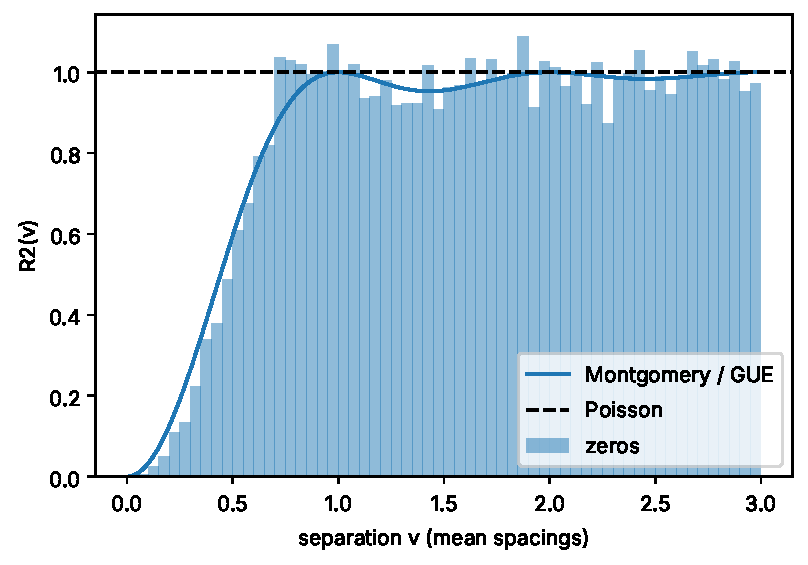
\includegraphics[width=0.85\linewidth]{figs/level-statistics_paircorr.pdf}
\caption{Pair correlation of the first $10^4$ unfolded zeros: histogram of all differences $u_m-u_n$ with $0<u_m-u_n<3$ (bin width $0.05$), divided by the number of reference zeros and the bin width, against Montgomery's form $1-(\sin\pi v/\pi v)^2$ and the Poisson value $1$. The separation $v$ is in units of the mean spacing.}
\label{fig:level-statistics-paircorr}
\end{figure}

\begin{keyideas}
\item $R_2(v)$ counts all other levels at distance $v$; Poisson gives $R_2=1$; for small $v$, $R_2\approx p$.
\item Large-$N$ GUE: $R_2(v)=1-(\sin\pi v/\pi v)^2$ (theorem, proof in \cite{mehta}).
\item For the zeros: Montgomery's theorem (assuming RH, restricted test functions), the pair correlation conjecture (open), Odlyzko's numerical agreement \cite{odlyzko87}.
\end{keyideas}

%=====================================================================
\section{The Riemann zeros as a GUE-like spectrum}\label{sec:level-statistics-zeros}

\subsection{Reproducing paper Fig.~2}

You now have every tool needed to reproduce the paper's Fig.~2.

\begin{pycode}
import numpy as np, qmnt
import matplotlib.pyplot as plt
t = qmnt.zeros(10000)            # first 10^4 zeros
u = qmnt.Nsm(t)                  # unfold with paper Eq. (1)
ds = np.diff(u)                  # 9999 unfolded spacings
print(ds.mean(), ds.var(), np.mean(ds < 0.1))
s = np.linspace(0, 3.5, 400)
plt.hist(ds, bins=np.linspace(0, 3.5, 36), density=True)
plt.plot(s, 32/np.pi**2 * s**2 * np.exp(-4*s**2/np.pi), label="GUE")
plt.plot(s, np.pi/2 * s * np.exp(-np.pi*s**2/4), ":", label="GOE")
plt.plot(s, np.exp(-s), "--", label="Poisson")
plt.legend(); plt.xlabel("unfolded spacing s"); plt.ylabel("p(s)")
plt.savefig("gue.pdf")
\end{pycode}

Three lines do all the physics: \texttt{qmnt.zeros} supplies the data, \texttt{qmnt.Nsm} unfolds them with paper Eq.~(1), and \texttt{np.diff} forms the spacings. Everything else is plotting. When you run it you should find three things. First, a mean spacing within $2\times10^{-4}$ of one. Eq.~\eqref{eq:level-statistics-meanone} explains this: the mean of all 9999 spacings is exactly $1+(\delta_{10000}-\delta_1)/9999$, and both end fluctuations are observed to be below one in size. Second, a variance closer to the GUE value $0.178$ than to the GOE value $0.273$, and far from the Poisson value $1$. Third, a fraction of spacings below $0.1$ that is below $0.01$, far smaller than the Poisson fraction $0.0952$. Figure~\ref{fig:level-statistics-gue} shows the result. It is the paper's Fig.~2 recomputed, with the GOE surmise added for comparison (the paper shows only the GUE and Poisson curves).

\begin{figure}[htbp]\centering
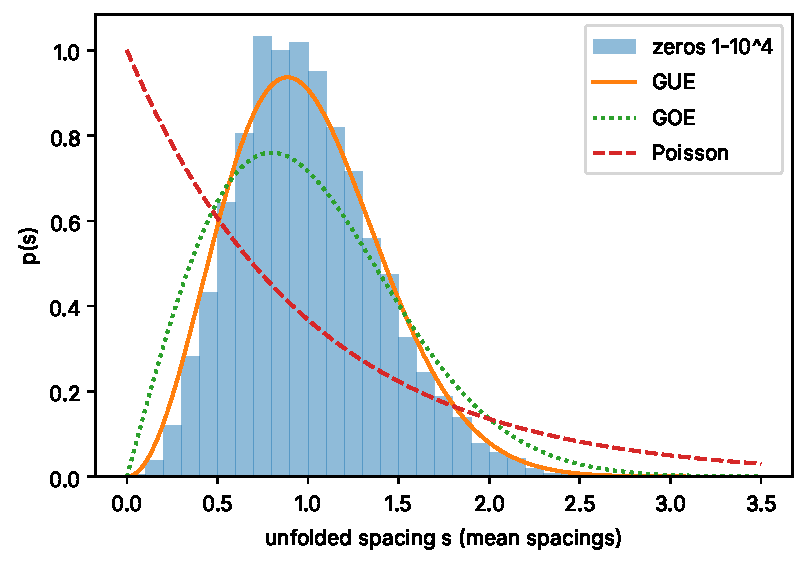
\includegraphics[width=0.85\linewidth]{figs/level-statistics_gue.pdf}
\caption{Reproduction of paper Fig.~2: histogram of the $9999$ unfolded nearest-neighbor spacings of the first $10^4$ zeros (unfolded with paper Eq.~(1)), against the GUE Wigner surmise $\frac{32}{\pi^2}s^2e^{-4s^2/\pi}$ (solid), the GOE surmise (dotted) and the Poisson law $e^{-s}$ (dashed). Spacings are in units of the local mean spacing.}
\label{fig:level-statistics-gue}
\end{figure}

Why does the paper include this figure at all? Not as evidence about operators, but as a \emph{dataset check}. If the zeros had been computed wrongly (a zero missed, a zero duplicated, a precision problem), the histogram would show it at once. A missed zero produces a spacing near $2$, which GUE makes very rare; a duplicated zero produces a spacing $0$, which GUE forbids. If the unfolding function had the wrong density (for example a wrong factor in the logarithmic term), the mean spacing would drift away from one and the histogram would be distorted. A wrong additive constant, such as an error in the $\tfrac78$, would however cancel in every spacing and go unnoticed. A clean match to the surmise therefore confirms ``the dataset and unfolding'' (paper Sec.~II A).

\subsection{What GUE statistics do and do not imply}

It is tempting to read Fig.~\ref{fig:level-statistics-gue} as saying ``the zeros are the eigenvalues of some Hermitian operator without time-reversal symmetry''. Be careful. Here is the status of each statement.
\begin{itemize}
\item \textbf{Numerical observation:} the statistics of the unfolded zeros agree closely with GUE statistics \cite{odlyzko87}.
\item \textbf{Theorem (conditional):} Montgomery's restricted pair correlation result, assuming RH \cite{montgomery}.
\item \textbf{Heuristic/hope:} that this agreement points toward a self-adjoint operator whose eigenvalues are the $t_n$ (Hilbert--P\'olya idea, Chapter~\ref{ch:hilbert-polya}). This is open.
\item \textbf{Not implied:} any \emph{specific} operator. A GUE matrix of the right size, unfolded, has, to the accuracy of the comparisons above, the same local statistics as the zeros, yet its individual eigenvalues have nothing to do with the individual zeros.
\end{itemize}
The last point is precisely the gap between statistics and positions that the paper exploits. Statistics are invariant under a vast set of changes to the spectrum: reflect it, shift it by a fraction of a spacing, replace it by another random draw, and the histogram does not change. A model can therefore reproduce the statistics, even reproduce the training zeros themselves, and still predict nothing about the next zero. Predicting position is a much more demanding test, and it is the test the paper applies (Chapter~\ref{ch:generalization}).

\begin{pitfall}
``Has GUE statistics'' is a property shared by every generic complex Hermitian random matrix. It cannot single out one operator. Do not quote a matching spacing histogram as evidence that a particular fitted Hamiltonian ``is'' the zeta operator.
\end{pitfall}

\subsection{Negative correlations of consecutive fluctuations}

Look again at the column $\delta_n$ of Table~\ref{tab:level-statistics-re1}: $-0.051,+0.070,-0.107,+0.171,-0.183,\dots$ In this short sample of ten values the signs mostly alternate: a zero pushed above its smooth position tends to be followed by one pushed below. Ten values are only suggestive. Fig.~\ref{fig:level-statistics-acf} below measures the effect over 400 zeros, and the paper reports the same thing (negative autocorrelation at lags 1--3, paper Sec.~III). This is a \textbf{numerical observation} about the low zeros, not something we derive. In particular it is \emph{not} a consequence of level repulsion alone. If zero $n$ moves up and repels zero $n+1$, then zero $n+1$ is pushed up as well, which by itself would favor a \emph{positive} correlation of consecutive fluctuations. What we can do exactly is relate the sign of the correlation to two measurable quantities, through the identity below.

We can quantify it. Recall from Chapter~\ref{ch:probability} that the autocovariance at lag $k$ of a sequence with mean zero is $C_k=\langle\delta_n\delta_{n+k}\rangle$, and the autocorrelation is $r_k=C_k/C_0$. The sequence is called \textbf{stationary} when averages such as $\langle\delta_n\rangle$ and $\langle\delta_n\delta_{n+k}\rangle$ do not depend on $n$, so that $C_k$ depends only on the lag $k$. The unfolded spacing is $\Delta u_n=1+\delta_{n+1}-\delta_n$ (from Eq.~\eqref{eq:level-statistics-delta}), so
\begin{align}
\mathrm{Var}(\Delta u)&=\left\langle(\delta_{n+1}-\delta_n)^2\right\rangle\nonumber\\
&=\langle\delta_{n+1}^2\rangle-2\langle\delta_{n+1}\delta_n\rangle+\langle\delta_n^2\rangle\nonumber\\
&=2\left(C_0-C_1\right).
\label{eq:level-statistics-varlink}
\end{align}
This is an identity, valid for any stationary sequence. Solved for $C_1$ it reads
\begin{equation}
C_1=C_0-\tfrac12\mathrm{Var}(\Delta u),
\label{eq:level-statistics-C1}
\end{equation}
so the lag-1 covariance is negative exactly when the fluctuation variance $C_0$ is smaller than half the spacing variance. For the first thousand zeros, computing both sides with qmnt (unfold as in the listing of Sec.~\ref{sec:level-statistics-unfolding}), this is what happens: $C_0<\tfrac12\mathrm{Var}(\Delta u)$, so $C_1<0$, and the spacings vary more than $2C_0$ alone would give. Nothing forces this in general.

\begin{beyond}
For large GUE matrices the variance of the fluctuations $\delta_n$ grows slowly (logarithmically) with the matrix size, while the variance of the unfolded spacings stays near $0.178$. By Eq.~\eqref{eq:level-statistics-C1}, $C_1$ then becomes positive. We quote this growth without derivation; see \cite{mehta}.
\end{beyond}

So the negative lag-1 correlation is a property of the zeros at the heights studied here, not a universal consequence of repulsion.

\textbf{Consecutive spacings.} The alternation of long and short spacings noticed in Table~\ref{tab:level-statistics-re1} is measured by the covariance of consecutive spacings. The mean spacing is one, so $\mathrm{Cov}(\Delta u_n,\Delta u_{n+1})=\langle(\Delta u_n-1)(\Delta u_{n+1}-1)\rangle$, and $\Delta u_n-1=\delta_{n+1}-\delta_n$. Hence
\begin{align}
\mathrm{Cov}(\Delta u_n,\Delta u_{n+1})&=\left\langle(\delta_{n+1}-\delta_n)(\delta_{n+2}-\delta_{n+1})\right\rangle\nonumber\\
&=\langle\delta_{n+1}\delta_{n+2}\rangle-\langle\delta_{n+1}^2\rangle-\langle\delta_n\delta_{n+2}\rangle+\langle\delta_n\delta_{n+1}\rangle\nonumber\\
&=C_1-C_0-C_2+C_1\quad\text{(stationarity)}\nonumber\\
&=-C_0+2C_1-C_2 .
\label{eq:level-statistics-spacingcov}
\end{align}
The term $-C_0$ is always negative, and $2C_1$ is negative whenever $C_1<0$. For the first thousand zeros, computed with qmnt, the correlation of consecutive unfolded spacings is negative: a long spacing tends to be followed by a short one. The sample value of the left side of Eq.~\eqref{eq:level-statistics-spacingcov} agrees with $-C_0+2C_1-C_2$ computed from the same zeros to better than $0.01$. This is the spacing counterpart of the negative fluctuation autocorrelation that the paper reports at lags 1--3.

\textbf{A simple model that shows the consequence.} Let $\varepsilon_n$ be independent random numbers with mean zero and variance $\sigma^2$, and let
\begin{equation}
\delta_n=\varepsilon_n-\alpha\,\varepsilon_{n-1},\qquad 0<\alpha\le1 .
\label{eq:level-statistics-ma1}
\end{equation}
Because different $\varepsilon$'s are uncorrelated, only matching indices contribute to averages of products:
\begin{align}
C_0&=\langle(\varepsilon_n-\alpha\varepsilon_{n-1})^2\rangle=\sigma^2+\alpha^2\sigma^2=(1+\alpha^2)\sigma^2,\\
C_1&=\langle(\varepsilon_n-\alpha\varepsilon_{n-1})(\varepsilon_{n+1}-\alpha\varepsilon_n)\rangle=-\alpha\langle\varepsilon_n^2\rangle=-\alpha\sigma^2,\\
C_2&=\langle(\varepsilon_n-\alpha\varepsilon_{n-1})(\varepsilon_{n+2}-\alpha\varepsilon_{n+1})\rangle=0 .
\end{align}
So $r_1=-\alpha/(1+\alpha^2)<0$ and $r_k=0$ for $k\ge2$.

Now suppose you know $\delta_{n-1}$ and $\delta_{n+1}$ and ``interpolate smoothly'' by predicting $\hat\delta_n=\tfrac12(\delta_{n-1}+\delta_{n+1})$. How well does $\hat\delta_n$ correlate with the truth $\delta_n$? Using the definitions of Chapter~\ref{ch:probability}:
\begin{align}
\mathrm{Cov}(\delta_n,\hat\delta_n)&=\tfrac12\left(\langle\delta_n\delta_{n-1}\rangle+\langle\delta_n\delta_{n+1}\rangle\right)=\tfrac12(C_1+C_1)=C_1,\\
\mathrm{Var}(\hat\delta_n)&=\tfrac14\left(C_0+2C_2+C_0\right)=\tfrac12C_0\quad(C_2=0),\\
\corr(\delta_n,\hat\delta_n)&=\frac{C_1}{\sqrt{C_0\cdot\tfrac12C_0}}=\sqrt2\,r_1=-\frac{\sqrt2\,\alpha}{1+\alpha^2}.
\label{eq:level-statistics-interpcorr}
\end{align}
For $\alpha=1$ this is $-0.707$. The prediction made from the nearest neighbors points in the \emph{wrong direction}. Smooth interpolation, which assumes that nearby values are similar, is anticorrelated with a sequence whose nearby values are dissimilar.

\begin{sample}{The neighbor-average predictor}
In the model of Eq.~\eqref{eq:level-statistics-ma1} with $\alpha=0.6$, find $r_1$ and the correlation of the neighbor average with the truth.

\textbf{Step 1:} $r_1=-0.6/(1+0.36)=-0.6/1.36=-0.441$.

\textbf{Step 2:} By Eq.~\eqref{eq:level-statistics-interpcorr}, $\corr=\sqrt2\times(-0.441)=-0.624$.

\textbf{Answer:} \[\boxed{r_1=-0.441,\quad \corr(\delta_n,\hat\delta_n)=-0.624}\]
\end{sample}

The real zeros are more complicated (their autocorrelation is negative at several lags and contains the slow oscillations of the prime sum, Chapter~\ref{ch:explicit-formula}), but the mechanism is the same. The paper reports exactly this: ``the fluctuation sequence has negative autocorrelation at lags 1--3, so any smooth interpolation between neighbouring training levels is anticorrelated with the truth (the mean of the two nearest training fluctuations gives $-0.26$ to $-0.41$)'' (paper Sec.~III, ``Within-height splits''). Figure~\ref{fig:level-statistics-acf} shows the autocorrelation of $\delta_n$ for zeros 1--400.

\begin{figure}[htbp]\centering
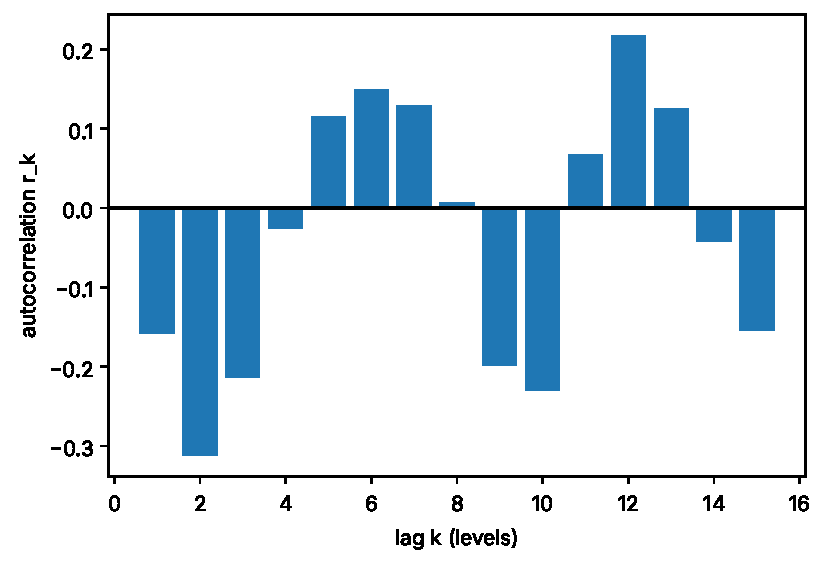
\includegraphics[width=0.85\linewidth]{figs/level-statistics_acf.pdf}
\caption{Autocorrelation $r_k$ of the fluctuations $\delta_n=(t_n-s_n)/\gap_n$ (in mean spacings) of zeros 1--400, for lags $k=1,\dots,15$. The first lags are negative: consecutive zeros tend to be displaced in opposite directions from their smooth positions.}
\label{fig:level-statistics-acf}
\end{figure}

\begin{checkpoint}
If consecutive fluctuations were \emph{positively} correlated ($r_1>0$, $r_2=0$), would the neighbor average be correlated or anticorrelated with the truth?
\end{checkpoint}
\checkanswer{Correlated: Eq.~\eqref{eq:level-statistics-interpcorr} gives $\corr=\sqrt2\,r_1>0$. The sign of the interpolation's skill follows the sign of the lag-1 correlation.}

\begin{keyideas}
\item Paper Fig.~2 is reproduced in a few lines; it validates the data and the unfolding.
\item GUE statistics are a numerical observation; they do not identify an operator and say nothing about individual positions.
\item For the low zeros, consecutive fluctuations are observed to be negatively correlated (a numerical observation, not derived from repulsion). Whenever $r_1<0$ and $r_2\approx0$, neighbor interpolation is anticorrelated with the truth ($\corr=\sqrt2\,r_1$ in the MA(1) model, Eq.~\eqref{eq:level-statistics-interpcorr}).
\end{keyideas}

%=====================================================================
\section{Paper connection}\label{sec:level-statistics-paper}

\textbf{Sec.~I, first paragraph.} ``Montgomery's pair-correlation theorem and Odlyzko's numerics match Gaussian unitary ensemble (GUE) eigenvalue statistics \cite{montgomery,odlyzko87}.'' You can now unpack this: the theorem is Montgomery's conditional, restricted result on $R_2$ (Sec.~\ref{sec:level-statistics-pair}); the numerics are Odlyzko's spacing and pair-correlation histograms; GUE is the ensemble of Sec.~\ref{sec:level-statistics-wigner}. The paper calls this ``circumstantial evidence'', which is the honest status.

\textbf{Sec.~II A and Fig.~2.} ``Unfolded spacings of the first $10^4$ zeros show textbook GUE level repulsion (Fig.~2), confirming the dataset and unfolding.'' The unfolding is Eq.~\eqref{eq:level-statistics-unfold} with paper Eq.~(1); the curves in the caption are Eqs.~\eqref{eq:level-statistics-gue} and~\eqref{eq:level-statistics-poisson}; you reproduced the figure in Sec.~\ref{sec:level-statistics-zeros}. Its role is validation, not argument.

\textbf{The unit of every rms.} ``All errors below are quoted in units of the local mean spacing $\gap_n=ds_n/dn$'' (Sec.~II A). Measuring in mean spacings is unfolding (Eq.~\eqref{eq:level-statistics-flucequiv}). That is why errors at zero 400 and zero $10^4$ can be compared in Table~V, and why the null grows only mildly, from $0.263$ to $0.296$ (Table~V; Sec.~II C, ``Within-height splits'').

\textbf{Sec.~III, ``Within-height splits''.} The paper observes negative autocorrelation at lags 1--3; this is a numerical observation, which Fig.~\ref{fig:level-statistics-acf} reproduces for zeros 1--400. Given that observation, Sec.~\ref{sec:level-statistics-zeros} shows why neighbor interpolation is anticorrelated with the truth (Eq.~\eqref{eq:level-statistics-interpcorr} in the simple model), which accounts for the paper's neighbor-mean correlation of $-0.26$ to $-0.41$. This chapter does not derive the negative autocorrelation itself from repulsion. The paper uses this to call the negative correlations of Table~III at $M\le200$ ``mechanical''.

\textbf{Sec.~V, ``The proposed mechanism fails quantitatively''.} The dominant $p=2$ oscillation has period $2\pi/\log2\approx9$ in $t$, ``only $\sim$6--7 levels at these heights''. Dividing a period in $t$ by the mean spacing (Eq.~\eqref{eq:level-statistics-gap}) is again unfolding (Problem 17).

\textbf{What this chapter does \emph{not} support.} Nothing in Fig.~2 bears on whether a fitted potential predicts. Statistics are shared by all GUE-like spectra; the paper's test (held-out positions, Figs.~1, 3, Tables I--V) is of a different and stronger kind.

%=====================================================================
\section{Summary}\label{sec:level-statistics-summary}
\begin{itemize}
\item Unfolding $u_n=\bar N(E_n)$ gives unit mean spacing (Eqs.~\eqref{eq:level-statistics-unfold}, \eqref{eq:level-statistics-meanone}); for the zeros the mean gap is $2\pi/\log(t/2\pi)$ (Eq.~\eqref{eq:level-statistics-gap}), and $\delta_n\approx(t_n-s_n)/\gap_n$ (Eq.~\eqref{eq:level-statistics-flucequiv}).
\item Spacing densities obey $\int p=\int sp=1$ (Eq.~\eqref{eq:level-statistics-twoconditions}).
\item Independent levels: $p_{\rm P}=e^{-s}$ (Eq.~\eqref{eq:level-statistics-poisson}); mean 1, variance 1.
\item $2\times2$ spacing $\sqrt{(a-d)^2+4b^2}$ (Eq.~\eqref{eq:level-statistics-2x2gap}); avoided crossings.
\item Wigner surmises: $p_{\rm GOE}=\frac\pi2se^{-\pi s^2/4}$, $p_{\rm GUE}=\frac{32}{\pi^2}s^2e^{-4s^2/\pi}$ (Eqs.~\eqref{eq:level-statistics-goe}, \eqref{eq:level-statistics-gue}); variances $0.273$, $0.178$.
\item GUE pair correlation $1-(\sin\pi v/\pi v)^2$ (Eq.~\eqref{eq:level-statistics-montgomery}); Montgomery (conditional, restricted), conjecture open, Odlyzko numerics.
\item $\mathrm{Var}(\Delta u)=2(C_0-C_1)$ (Eq.~\eqref{eq:level-statistics-varlink}) and $\mathrm{Cov}(\Delta u_n,\Delta u_{n+1})=-C_0+2C_1-C_2$ (Eq.~\eqref{eq:level-statistics-spacingcov}); for the low zeros $C_1<0$ is observed, not derived from repulsion; neighbor interpolation has $\corr=\sqrt2r_1$ in the MA(1) model (Eq.~\eqref{eq:level-statistics-interpcorr}).
\end{itemize}

%=====================================================================
\section{Problems}\label{sec:level-statistics-problems}
\begin{problemlist}
\prob{1}{Unfold the box levels $E_k=(k\pi/2L)^2$ for the scale-2 box $L=59.957$. What are the unfolded spacings?}
\prob{1}{For Poisson levels, what is the probability that a spacing exceeds 1?}
\prob{1}{Find the mean spacing of the zeros at $t=100$ from Eq.~\eqref{eq:level-statistics-gap}.}
\prob{2}{For the GOE surmise, find $\Pr(s>1)$ exactly.}
\prob{2}{Let $U$ be a complex $2\times2$ matrix with $U^\dagger U=I$. Show that $\mathrm{tr}\big((UHU^\dagger)^2\big)=\mathrm{tr}(H^2)$ for every Hermitian $H$, so that the exponent $-\mathrm{tr}(H^2)/2\sigma_0^2$ of the GUE density does not depend on the basis.}
\prob{2}{Using the small-$\varepsilon$ law, estimate $\Pr(s<0.2)$ under GUE.}
\prob{2}{For $H(\tau)$ with $g=0.2$, find the minimum separation of the levels and the separation at $\tau=0.5$.}
\prob{2}{Compare the small-$v$ coefficients of $R_2$ for GUE and of $p_{\rm GUE}$. By what percentage do they differ?}
\prob{2}{In the model of Eq.~\eqref{eq:level-statistics-ma1} with $\alpha=0.5$, compute $r_1$ and the neighbor-average correlation.}
\prob{2}{Show that if spacings were exactly 1 (picket fence), $\delta_n$ would be constant and $\mathrm{Var}(\Delta u)=0$; check against Eq.~\eqref{eq:level-statistics-varlink}.}
\prob{3}{A symplectic degeneracy needs five conditions, so $p(s)=As^4e^{-Bs^2}$. Using Eq.~\eqref{eq:level-statistics-twoconditions} find $A$ and $B$.}
\prob{2}{Using qmnt, compute the variance of the unfolded spacings of zeros 1--1000 and of zeros 9001--10000. Does it drift toward the GUE value?}
\prob{2}{Using numpy, throw $2\times10^4$ uniform points on $[0,2\times10^4]$, sort, and compute the fraction of spacings below $0.1$. Compare with theory.}
\prob{3}{Using numpy, build a $400\times400$ GUE matrix ($H=(G+G^\dagger)/2$ with $G$ complex Gaussian), take the central 100 eigenvalues, unfold by dividing spacings by their mean, and compare the variance with $0.178$.}
\prob{1}{The paper's null rms on zeros 401--500 is $0.263$ (Sec.~II C). In the language of this chapter, what quantity's rms is this?}
\prob{2}{Paper Fig.~2 compares with GUE, not GOE. Which feature of the histogram near $s=0$ would distinguish the two?}
\prob{2}{Using qmnt, find the mean gap at $t_{400}$ and the number of levels in one period $2\pi/\log2$ of the $p=2$ wave (RE2). Compare with the paper's ``6--7 levels'' (Sec.~V).}
\prob{3}{Using qmnt, compute $\corr(\delta_n,\tfrac12(\delta_{n-1}+\delta_{n+1}))$ for $n=2,\dots,399$ and compare with the paper's range $-0.26$ to $-0.41$ (Sec.~III).}
\prob{2}{A spectrum is obtained by reflecting the unfolded zeros ($u\to-u$). Does its spacing histogram change? Can it predict the zeros? What does this say about Fig.~2?}
\prob{1}{Estimate $\Pr(s<0.05)$ for GUE using the small-$\varepsilon$ law.}
\prob{3}{In the model of Eq.~\eqref{eq:level-statistics-ma1}, use Eqs.~\eqref{eq:level-statistics-varlink} and~\eqref{eq:level-statistics-spacingcov} to show that the correlation of consecutive unfolded spacings is $-(1+\alpha)^2/[2(1+\alpha+\alpha^2)]$, and evaluate it for $\alpha=1$.}
\prob{2}{Verify $I_2(B)=\sqrt\pi/(4B^{3/2})$ numerically for $B=4/\pi$.}
\end{problemlist}

%=====================================================================
\section{Answers to selected problems}\label{sec:level-statistics-answers}
\textbf{1.} $\bar N(E)=2L\sqrt E/\pi-\tfrac12$ gives $u_k=k-\tfrac12$; every $\Delta u_k=1$ and every $\delta_k=0$, independent of $L$.

\textbf{2.} $Q(1)=e^{-1}=0.368$.

\textbf{3.} $\log(100/2\pi)=\log15.9155=2.7674$; $\gap=2\pi/2.7674=2.270$.

\textbf{5.} $(UHU^\dagger)^2=UHU^\dagger UHU^\dagger=UH(U^\dagger U)HU^\dagger=UH^2U^\dagger$. With $\mathrm{tr}(XY)=\mathrm{tr}(YX)$ for $X=U$, $Y=H^2U^\dagger$: $\mathrm{tr}(UH^2U^\dagger)=\mathrm{tr}(H^2U^\dagger U)=\mathrm{tr}(H^2)$.

\textbf{7.} $\pm\sqrt{\tau^2+g^2}$: minimum $2g=0.4$; at $\tau=0.5$, $2\sqrt{0.29}=1.077$.

\textbf{9.} $r_1=-0.5/1.25=-0.4$; $\corr=\sqrt2(-0.4)=-0.566$.

\textbf{11.} $I_5=\frac{4}{2B}I_3=\frac{1}{B^3}$, so $A=B^3$; then $AI_4=\frac{3\sqrt\pi}{8}B^{1/2}=1$, $B=\frac{64}{9\pi}=2.264$, $A=\left(\frac{64}{9\pi}\right)^3=\frac{2^{18}}{3^6\pi^3}=11.60$.

\textbf{13.} The fraction should be near $1-e^{-0.1}=0.0952$, within about $0.004$ (binomial standard error $\sqrt{0.095\times0.905/(2\times10^4)}\approx0.002$).

\textbf{15.} The rms over zeros 401--500 of the fluctuation $\delta_n=(t_n-s_n)/\gap_n$, i.e.\ of unfolded deviations from the smooth positions.

\textbf{17.} \texttt{qmnt.zeros(400)[-1]} gives $t_{400}\approx680$. Eq.~\eqref{eq:level-statistics-gap} then gives $\gap\approx1.341$ (it changes by only about $0.0004$ per unit of $t$ here), and one period of RE2 spans $9.065/1.341\approx6.8$ levels, inside ``6--7''.

\textbf{19.} Reflection reverses the order of spacings but keeps the multiset of spacings, so the histogram is unchanged; the reflected positions are useless for predicting the zeros. Fig.~2 tests the statistics, not positions.

\textbf{20.} $\frac{32}{3\pi^2}(0.05)^3=1.351\times10^{-4}$.

\textbf{21.} From the text, $C_0=(1+\alpha^2)\sigma^2$, $C_1=-\alpha\sigma^2$, $C_2=0$. Then $\mathrm{Cov}=-C_0+2C_1-C_2=-(1+\alpha^2+2\alpha)\sigma^2=-(1+\alpha)^2\sigma^2$ and $\mathrm{Var}(\Delta u)=2(C_0-C_1)=2(1+\alpha+\alpha^2)\sigma^2$. The ratio is $-(1+\alpha)^2/[2(1+\alpha+\alpha^2)]$; for $\alpha=1$ it is $-4/6=-0.667$.
